\chapter{Evaluation}\label{ch:evaluation}
% take a step back and put your results from 4 into context.
This chapter represents the evaluation phase, which includes the evaluation, demonstration and
communication activities outlined in the \ac{DSR} process in \cref{ch:research-methodology}.

The evaluation activity provides a comprehensive analysis of the Machine Learning models built in the
previous chapter.
This phase evaluates the effectiveness of the developed models in solving the defined research questions.
During the demonstration phase, different scenarios are chosen to illustrate the potential real-world applications of
the models and their performance in these contexts.
Finally, during the communication phase, the results of this study will be presented with the aim of effectively
communicate the results and their interpretation.

The \cref{tab:evaluation_criteria} provides an overview of the quality metrics employed for the evaluation.
They are structured based on the \ac{GQM} approach discussed in \cref{sec:goal-question-metric-approach}.
The quality metrics align with the quality model from~\cite{siebert2022construction}, which in turn is based on
the ISO/IEC 9126 standard for software quality evaluation.
This standard has been adapted by~\cite{siebert2022construction} to address the specific requirements of Machine
Learning models, as detailed in~\cref{sec:evaluation-of-machine-learning-models}.
Since~\cite{siebert2022construction} primarily focus on evaluating classification models, the quality metrics have
been tailored to suit the needs of the regression models implemented in this study.
Each individual quality metric section provides further elaboration, on what was changed.
The \cref{tab:evaluation_criteria} also displays the quality metrics used for evaluating the \ac{ML} models.

\captionsetup{margin={5pt,5pt}}
\begin{table}[H]
    \begin{tcolorbox}[arc=0pt,boxrule=0.5pt]
        \centering
        {\renewcommand{\arraystretch}{1}
            \begin{tabular}{p{2cm}p{8cm}p{3cm}}
                \toprule
                \thead{\textbf{Goal}} & \thead{\textbf{Question}}
                & \thead{\textbf{Metric}} \\
                \toprule
                \textbf{Correctness} &
                How good is the ability of the model to to predict the spring back?
                ~\cite[p. 16]{siebert2022construction}?
                &
                MAE, \newline MSE, \newline RMSE
                \\
                \hdashline
                \textbf{Relevance} &
                Does the bias-variance tradeoff work well for the model?
                The model should neither overfit or underfit.
                ~\cite[p. 16]{siebert2022construction}?
                & Variance of CV, \newline $R^2$
                \\
                \hdashline
                \textbf{Robustness} & Ability of the model to handle outliers, noise
                and other data quality issues~\cite[p. 16]{siebert2022construction}
                & Missing Values Test, \newline Noise Test
                \\
                \hdashline
                \textbf{Stability} & Does the artifact generate repeatable
                results when trained on different data-sets?~\cite[p. 16]{siebert2022construction}
                & LOOCV stability
                \\
                \hdashline
                \textbf{Interpret-\newline ability} & How well can the model be
                explained?~\cite[p. 16]{siebert2022construction}
                & Different interpretability methods
                \\
                \hdashline
                \textbf{Resource utilization} & How much resources are
                required to train and run
                the model?~\cite[p. 16]{siebert2022construction}
                & Training time, \newline runtime, \newline storage space
                \\
                \bottomrule
            \end{tabular}
        } % renew command
    \end{tcolorbox}
    \caption{Overview of the goals, questions and metrics for the
    evaluation of artifacts
    following the \ac{GQM} approach.}
    \label{tab:evaluation_criteria}
\end{table}


\section{DP1: Correctness}\label{sec:dp1:-correctness}
% Ability of the model to perform the current task measured on the
% development dataset and the
% runtime dataset

The model must be able to perform well on the selected task.
\cite{siebert2022construction} used the classification metrics precision, recall and F- score to evaluate the
correctness.
Since predicting the spring back is a regression task, these metrics are not applicable.
For this study metrics are needed to measure how well the predicted spring back for a specific observation
matches the actual spring back.
These metrics used in this study are the MAE, MSE and RMSE and where presented in~\cref{subsubsec:regression-metrics}
For the evaluation the \textit{sci-kit learn}~(\cite{scikit-learn}) implementations of these metrics were used.

There is an ongoing debate regarding the best metric to use for evaluating regression models.
For instance~\cite{willmott2005advantages} contend that the RMSE is not an appropriate measure for determining the
average performance of a model and suggest using the MAE instead, while~\cite{chai2014root} argue in favor of the RMSE.
The MAE is commonly used when a dataset contains outliers.
However, as the dataset of this study (reviewed in \cref{subsec:dataset-exploration}) is likely to not contain many
outliers, the
RMSE will be used as the primary metric in this study~\cite[p. 1249]{chai2014root}.
The MSE and MAE will be used as well but only when they make sense, for example when noise is added to the dataset
and therefore more outliers (\cref{sec:robustness}) are present or if the non squared error yields more meaningful
results.

Both measures will be included in the analysis, to give the reader a better understanding of the performance of
the models.
The MSE was not included in the analysis, as it is not expressed in the same unit as the data and is therefore
more difficult to interpret and might be misleading.
After selecting the metrics, the subsequent step is to determine an acceptable margin of error, which will be
addressed in the following chapter.

\subsection*{How much error is acceptable?}\label{subsec:how-much-error-is-acceptable}

A crucial aspect to consider when assessing the performance of a model is determining the acceptable margin of error.
The ISO 2768 standard outlines various levels of mechanical precision and associated tolerances, including those for
angular dimensions in formed metal components~\cite[pp. 1--3]{ISO2768}.
These tolerances are used to determine the acceptable margin of error for the model.

The standard distinguishes between different precision levels, with ``f'' (fine) being the highest, followed by ``m'' (
medium), ``c'' (coarse) and ``v'' (very coarse).
Additionally, the standard considers the side length of different parts, as this affects the tolerances
~\cite[p. 3]{ISO2768}.
Given that the metal sheets used in this study measure 80 mm in length and are bent in the middle, each side has a
length of 40 mm.
For metal parts with side lengths between 10 mm and 50 mm, the f and m tolerance levels for angular
dimensions are ±0°30' (degrees and minutes).
This equates to a ±0.5° tolerance for the opening angle.
The c and v levels are ±1° (degree) and ±2° (degrees) respectively.
This means that the model should be able to predict the spring back with an error of less than 0.5° to be considered
f or m.
This will be checked in the evaluation of the models which is done in the next \cref{subsec:results}.

\subsection{Results}\label{subsec:results}
The \cref{tab:results-correctness} presents the results of the evaluation of the \ac{ML} models for
the \ac{DP} correctness, sorted by the RMSE in ascending order.
The results where calculated using 5-fold cross validation and the mean of the RMSE as well as the MAE are presented.
It can be can be concluded that the best models have an RMSE of less than 0.2 millimetres.

The Linear Regression and Decision Tree models have poor predictive performance compared to the other models.
For the \ac{LR} model this is expected since the relationship between the independent and dependent variables is
not linear.
In contrast, Decision Trees can perform poorly when overfitting the training data and they are prone to
instability.
These problems are mitigated by using ensemble methods like Random Forest and Gradient Boosted Trees.
As the simple Decision Tree and Linear Regression models are not able to predict the spring back accurately enough,
they are not considered for the next steps of the evaluation.
As these are only two algorithms that are deemed interpretable, in~\cref{sec:interpretability} alternative techniques
will be identified for the interpretability assessment.

The Ada Boost, Random Forest, Gradient Boosted Tree, and Extra Tree models demonstrate moderate predictive
performance while the Multi-Layer-Perceptron and Support Vector Machine models have relatively low MAE
and RMSE values, indicating good predictive performance.
It is worth noting that the SVM model has a slightly better MAE while still maintaining a comparable RMSE compared
to the other models.
This could be because the errors made by the SVM are evenly distributed across instances or
because the errors made by the other models are large for a few instances but smaller for the rest.

% Table wit hall used machine learning models and their metrics
\begin{table}[H]
    \begin{tcolorbox}[arc=0pt,boxrule=0.5pt]
% \sisetup{group-minimum-digits = 4}
        \centering
        \begin{tabular}{lll}
            \toprule
            \thead{\textbf{Model Name}} & \thead{\textbf{MAE}}
            & \thead{\textbf{RMSE}} \\
            \toprule
            \textbf{Decision Tree}            & 0.275 & 0.401 \\
            \hdashline
            \textbf{Linear Regression}        & 0.228 & 0.283 \\
            \hdashline
            \textbf{Ada Boost}                & 0.250 & 0.293 \\
            \hdashline
            \textbf{Gradient Boosted Trees}   & 0.193 & 0.261 \\
            \hdashline
            \textbf{Random Forest}            & 0.220 & 0.277 \\
            \hdashline
            \textbf{Extra Trees }             & 0.216 & 0.261 \\
            \hdashline
            \textbf{Multi-Layered-Perceptron} & 0.161 & 0.205 \\
            \hdashline
            \textbf{Support Vector Machine}   & 0.128 & 0.170 \\
            \bottomrule
        \end{tabular}
    \end{tcolorbox}
    \caption{\textbf{Results for the DP 1 :} The results are sorted by RMSE in ascending
    order.}
    \label{tab:results-correctness}
\end{table}


As already noted most models have a RMSE below 0.2 which means that the error for a predicted spring back value is
0.2~mm.
For example if the spring back is 0.5 mm the models could predict values ranging from 0.3~mm to 0.7~mm.
In \cref{subsec:how-much-error-is-acceptable} it was stated that the tolerance for the spring back is 0.5\degree.
In \cref{tab:examples-tolerance} multiple samples from the dataset where chosen and their tolerance was calculated.
The samples where chosen with the goal to have a wide range of spring back values and different input values.
The \cref{sec:demonstration} describes in more detail why exactly these samples where chosen.

Since the spring back in the dataset was measured in millimetres but the tolerance is given in degrees the following
equation was applied to convert the spring back to degrees:

\begin{tcolorbox}[arc=0pt,boxrule=0.5pt]
    \begin{equation}
        \arctan\left(\frac{l/2}{y_p}\right)\cdot\frac{180}{\pi}
    \end{equation}
\end{tcolorbox}

Where $l$ is the support distance, which is the distance where the metal sheet is supported on the left and on the
right side in the experimental setup.
The results in \cref{tab:examples-tolerance} show that the tolerances for the chosen examples are between 0.09\degree and
0.27\degree which means that all of the examples are within the tolerance.
This means that the \ac{ML} models in this study are able to predict the spring back with an accuracy that is well
within the tolerance of the highest accuracy level (f) denoted in the DIN 2768.
That is enough for most applications used in the industry.

\begin{table}[H]
    \begin{tcolorbox}[arc=0pt,boxrule=0.5pt]
% \sisetup{group-minimum-digits = 4}
        \centering
        \begin{tabular}{ll}
            \toprule
            \textbf{Sample}            & \textbf{tolerance} \\
            $t$: 3 $V$: 20 $y_p$: 10   & \pm 0.27\degree    \\
            $t$: 3 $V$: 20 $y_p$: 20   & \pm 0.16\degree    \\
            \hdashline
            $V$: 20 $t$: 1.5 $y_p$: 10 & \pm 0.16\degree    \\
            $V$: 20 $t$: 1.5 $y_p$: 20 & \pm 0.09\degree    \\
            \hdashline
            $V$: 50 $t$: 0.5 $y_p$: 10 & \pm 0.18\degree    \\
            $V$: 50 $t$: 0.5 $y_p$: 20 & \pm 0.10\degree    \\
            \bottomrule
        \end{tabular}
    \end{tcolorbox}
    \caption{Calculation of the tolerance for chosen samples.}
    \label{tab:examples-tolerance}
\end{table}

The overall performance of the machine learning models are good and the best performing models are the
Support Vector Machine, Multi-Layer-Perceptron.
To further evaluate the performance of the models the relevance of the models is evaluated in the next section.


\section{DP2: Relevance}\label{sec:relevance}
% Does the model achieve a good bias-variance tradeoff? Which means neither
% overfitting or
% unterfitting the data.

% Bias variane trade-off
A model is considered relevant when it achieves a balance between bias and
variance, avoiding both overfitting and underfitting of the training data.
The relevance of the model can be quantified through by calculating variance of Cross-Validation, which proves insight
into how the model performs when trained and
evaluated on different subsets of data and how well it generalizes.

% Explanation interpretation of variance
A low variance indicates that the model's performance is consistent across
different folds, suggesting that the model is not overfitting the training data.
Conversely, a high variance implies that the performance can vary significantly
depending on the specific data points used in the test set, indicating a potential
overfitting problem.

A common metric for evaluating the effectiveness of regression models is the $R^2$ statistic, it shows how much of the
the variance is explained by the model.
It ranges usually from 0 to 1, where 0 means that the model does not explain any of the variance and a score of 1
means that the model fully explains the variance
~\cite[p. 43]{muller2016introduction}.
Therefore a higher $R^2$ score indicates a better fit for the model.

The equation \cref{eq:r2} shows the formula for the $R^2$ score as explained by
~\cite[p. 43]{muller2016introduction}.

\begin{tcolorbox}[arc=0pt,boxrule=0.5pt]
    \begin{equation}
        \label{eq:r2}
        R^2 = \frac{\text{Explained variance}}{\text{Total variance targert variable}}
    \end{equation}
\end{tcolorbox}

One unique feature of scikit-learn's implementation of $R^2$ is that the score can be negative if the model performs
poorly.
In the documentation of ~\cite{scikit-learn} it is noted, that a model would receive a $R^2$ score of 0.0 if it
consistently predicted the expected value of y regardless of the input features.
In order to achieve a negative $R2$ score with sci-kit learns' implementation a model has to perform worse than a
model that simply predicts the mean value of the dependend variable.
Therefore, a high $R^2$ score indicates a good model fit and a good bias-variance
tradeoff~\cite[p. 43]{muller2016introduction}.

\subsection{Results}\label{subsec:results3}

The \cref*{tab:results_relevance} displays the variance of cross-validation and the $R^2$ for all \ac{ML} algorithms,
sorted in ascending order of their $R^2$ score.
The variance of Cross-Validation was calculated using ccikit-learn's \texttt{cross\_val\_score} function and
five-fold cross-validation was used for the calculation.
The formula shown in \cref{eq:r2} was used to calculate the $R^2$ score.

It can be observed that most models have a relatively low variance, indicating that their performance is
consistent across different folds.
Based on the table the following models have the best bias-variance tradeoff:

\begin{enumerate}
    \item Support Vector Machine: The model has the highest $R^2$ value of 0.894 and a Variance of CV of
    0.016 which indictates that the model can explain a significant proportion of the variance in the data and
    performs consistently across different subsets of the data.
    \item Extra Trees: Comes second with an $R^2$ of 0.889 and a Variance of CV of 0.031, which is slightly higher
    than the Support Vector Machine.
    \item Multi-Layer Perceptron: The model has the third highest $R^2$ value of 0.825 and a low Variance
    of CV of 0.023, which implies that it can explain a substantial amount of variance in the data and
    performs consistently across different subsets.
    \item Random Forest: The Random Forest model has an $R^2$ value of 0.784 and a Variance of CV of 0.041.
\end{enumerate}


\begin{table}[h]
    \begin{tcolorbox}[arc=0pt,boxrule=0.5pt]
        \centering
        \begin{tabular}{lll}
            \toprule
            \thead{\textbf{Model Name}} & \thead{\textbf{Variance of CV}}
            & \thead{\textbf{$R^2$}} \\
            \toprule
            \textbf{Support Vector Machine} & 0.016 & 0.893 \\
            \hdashline
            \textbf{Extra Trees}            & 0.031 & 0.889 \\
            \hdashline
            \textbf{Multi-Layer-Perceptron} & 0.023 & 0.825 \\
            \hdashline
            \textbf{Random Forest}          & 0.041 & 0.784 \\
            \hdashline
            \textbf{Gradient Boosted Trees} & 0.021 & 0.761 \\
            \hdashline
            \textbf{Ada Boost}              & 0.072 & 0.676 \\
            \bottomrule
        \end{tabular}
    \end{tcolorbox}
    \caption{Results of DP 2 Relevance. The table shows the variance of cross-validation and the $R^2$ score for all
    models, sorted in ascending order of their $R^2$ score.}
    \label{tab:results_relevance}
\end{table}

The first two \ac{DP}s where conducted with the dataset in its original form. But what happens if the dataset is
manipulated and the data quality issues are introduced?
The following two \ac{DP}s where conducted with the dataset in its manipulated form.


\section{DP3: Robustness}\label{sec:robustness}
% Definition of robustness

Unlike \ac{DP} Correctness (\cref{sec:dp1:-correctness}), robustness is a non-functional characteristic of a \ac{ML}
model.
A way to evaluate the robustness is to check the correctness of the model with added noise to the
data
~\cite[p. 1]{saez2016evaluating}, if the model is still able to predict the correct values, it is
considered robust.
As mentioned in \cref{subsec:dataset-exploration} the data set was generated in a controlled environment and does not
contain many data quality issues and noise as they where removed during the process.
This offers the opportunity to test the robustness of the models by manipulating the data set to introduce the data
quality issues like missing values and noise.
To do that two tests where developed which are described in the following sections.

When applying a \ac{ML} model to real-world data, it is possible that some data is missing.
For example, there may be no data available for a specific die opening, which can be due to the die opening
was never being used before or a lack of recorded information.
On the other hand it is also possible that noise is present in the dataset.

To address these scenarios, the following tests where developed.

\subsection{Missing values}

Initially, the use of the \ac{LPOCV} method was considered.
However, this approach was omitted due to computational constraints, as it generates all possible
training and test sets by removing $p$ samples from the complete dataset, resulting in a large
number of overlapping test sets and a high computational cost.
As an alternative, regular CV was applied, with an increasing number of folds.
The minimum number of folds was two and the maximum was equal to the total number of samples in the
dataset.

Unfortunately, the experiment did not yield distinguishable results, indicating that all models performed similarly.
As a result, no conclusions could be drawn.
While various metrics were tested for the CV score, none provided any useful insights.
It is unclear why this particular test did not produce results, but it may have been due to the specific combination
of dataset and model used in this study.
Nevertheless, this approach remains a viable option for future research and should be considered.

The third and final experiment utilized random sampling to create different train-test data compositions, allowing
for the evaluation of the model's handling of missing data.
Split ratios from 90:10 to 10:90 were used, with a step size of 10.
This approach was inspired by a similar method used in a previous study~\cite[p. 570--574]{liu2021deep}  which used
thee different split ratios to evaluate the performance of a Deep Learning model.

The results of this experiment provided valuable insights into the model's performance under
different data compositions, particularly when dealing with missing
data and were used in conjunction with other metrics to gain a comprehensive understanding of
the model's overall performance.

The graph show in \cref{fig:results-missing-values} depicts the relationship between the size of the test set,
expressed as a
percentage
on the
x-axis, and
the RMSE achieved by the model on that particular test-train split, shown on the y-axis.
As expected, the plot reveals a decline in the model's performance as the amount of training data decreases, since the
model has less data to learn from and is therefore less accurate.
Initially, when the model is trained on 90\% of the data and tested on 10\%, only the GBT and MLP models perform well.
However, when trained on 80\% of the data, all models achieve good results, indicating that this test-train split is
optimal for all the models.
From this point on, the MLP consistently outperforms the other models, closely followed by the SVM model. The GBT
model also performs well overall, but its performance starts to deteriorate when the training data drops below 60\%,
lagging behind the other models.

The results show that having a small dataset doesn't necessarily mean that the results will be bad.
In fact, the results indicate that even with only 400 samples in the dataset, half of that would till produce good
results.
This implies that data quality plays a crucial role in determining the success of a model rather than the quantity of
data.
However, it is important to note that a dataset's size should not be too small, as that would be less than 200
samples in this case, which could lead to unreliable results.
The results show that even half of the only 400 sample string dataset would still yield good results.

\begin{figure}[h]
    \begin{tcolorbox}[arc=0pt,boxrule=0.5pt]
        \centering
        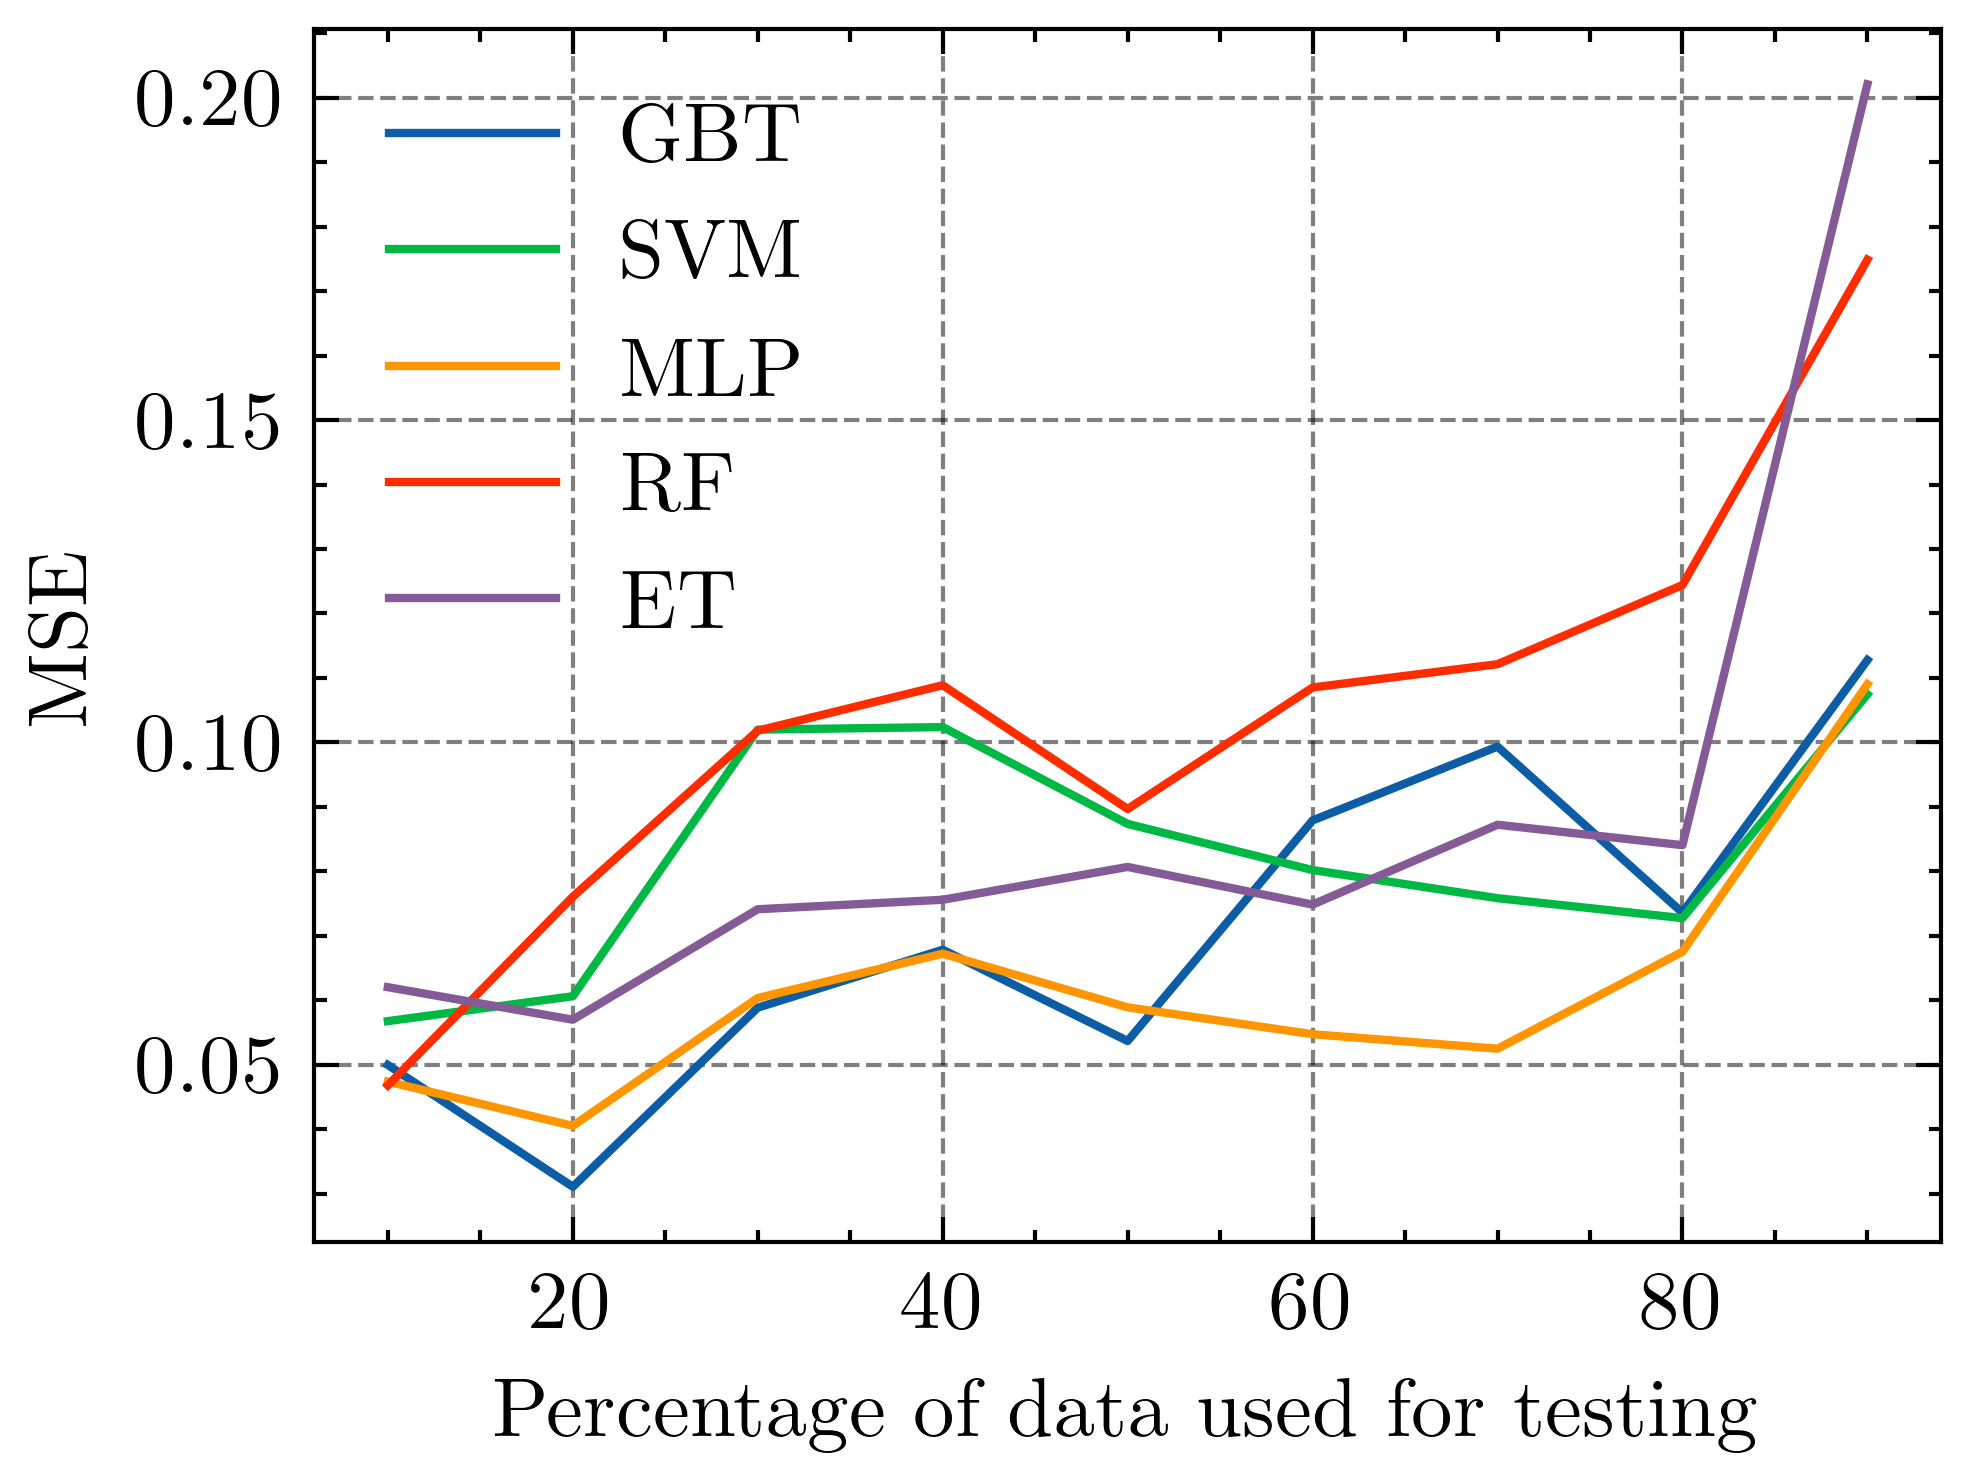
\includegraphics[width=0.6\textwidth]{chap5/images/missing_values_plot}
    \end{tcolorbox}
    \caption{Comparison of performance on less training data.}
    \label{fig:results-missing-values}
\end{figure}

After examining the variances depicted in \cref{fig:variance-missing-values}, it appears that the variances are
relatively small and the distinctions between the models are not particularly significant.
Still it can be seen that the the \ac{SVM} and \ac{MLP} models
perform the best and seem to be the most robust models when trained on less data.
It has to be noted, that as seen in the previous figure the most variance comes from training on
below 20\% of the data.

Overall the \ac{MLP} model seems to be the most robust model, as it performs well on all data
compositions and has the lowest variance.

\begin{figure}[h]
    \begin{tcolorbox}[arc=0pt,boxrule=0.5pt]
        \centering
        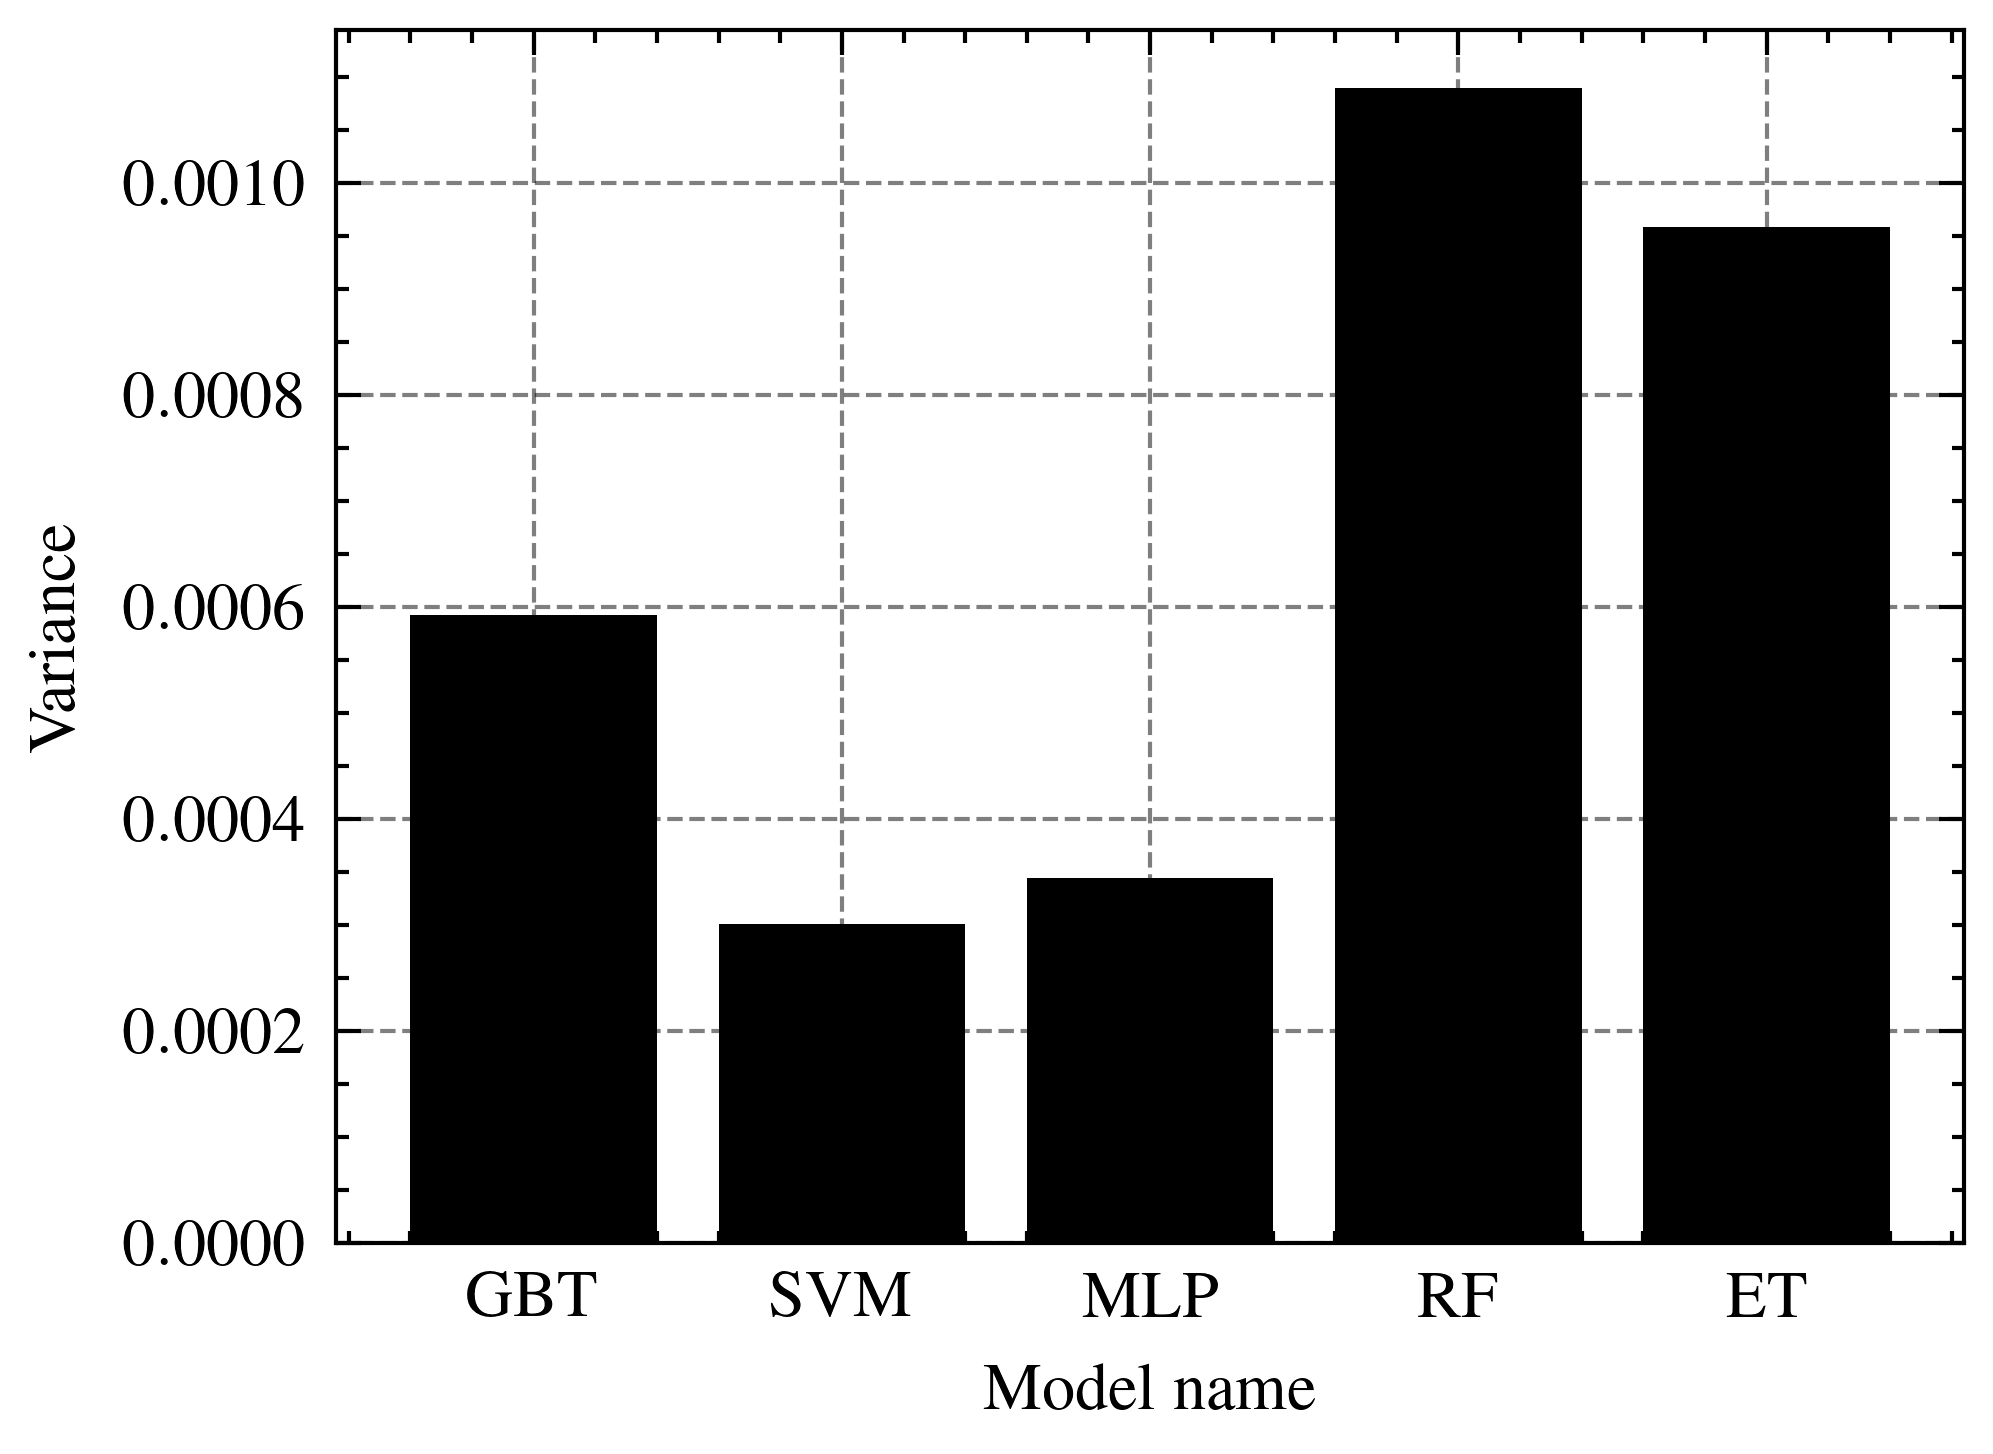
\includegraphics[width=0.6\textwidth]{chap5/images/variance_missing_values}
    \end{tcolorbox}
    \caption{Variance of models when trained on different data.}
    \label{fig:variance-missing-values}
\end{figure}

As previously noted not only missing values can be a problem in real world data, but also noise can be present in the
dataset.

\subsection{Noise}\label{subsec:noise}
A common practise in \ac{ML} is to add noise to the training data to evaluate
the model's generalization abilities.
In this study Gaussian Noise will be added to the data set to evaluate the robustness
of the models.
The noise will be added only the training data only as the test data should be as correct as possible to get
comparable results.
To add the noise, \textit{numpy.random.normal} function was used, which generates random numbers with a gaussian
distribution
(~\cite{harris2020array}).
The mean and standard deviation of each feature were calculated based on the original data.

To study the model's reaction to increasing amounts of noise, it was added
gradually to the data in increasing steps starting from 1\% to 50\%, which means that in the
last iteration contains as many noisy as `clean' samples.

\subsection{Results}\label{subsec:results-robustness}
The \cref{fig:results-noise-fig} presents the performance of models as more noise is introduced to the training
dataset.
The noisy dataset comprised 1000 samples, and the x-axis indicates the percentage of the original data that
was augmented with noise.
The dashed lines correspond to the default performance of the models in the absence of noise.
The results indicate that the performance of all models deteriorates rapidly with the addition of noise.
Specifically, the first 20\% of the noisy data causes the most significant decline in model performance, after which the
performance plateaus at a poor level.
It is noteworthy that the Extra Trees model exhibits the most robust performance, outperforming the Random Forest
and Gradient Boosted Trees models, which also demonstrate similar levels of resilience.

The results are interesting since they demonstrate that the typically high-performing SVM and MLP models
exhibit underperformance under the current conditions.
Specifically, the MLP is a highly expressive model with many parameters, making it prone to overfitting.
In this case, the addition of noise is likely causing the model to overfit to the noise, leading to poor
generalization performance.
On the other hand, the SVM aims to find an optimal hyperplane to separate the data with maximum margin, which makes
it highly sensitive to outliers and noise, making it challenging to identify the appropriate hyperplane.

These results emphasize the significance of selecting robust models and pre-processing the data to minimize the
presence of outliers.
Moreover, the study reveals that even a small amount of noise (i.e., 10\%) can significantly impact the model's
performance.
The significance of using a high-quality dataset is emphasized.
Also, the results indicate that the dataset used in this study is of high quality as the models perform well on the
default dataset but deteriorate rapidly when noise is added.
Additionally this test underlines the previous results, that relatively little data is enough to get good results.
This means that a good data quality outweighs a small dataset, as long as the dataset is not too small which would
be below 200 samples in this case.


\begin{figure}[h]
    \begin{tcolorbox}[arc=0pt,boxrule=0.5pt]
        \centering
        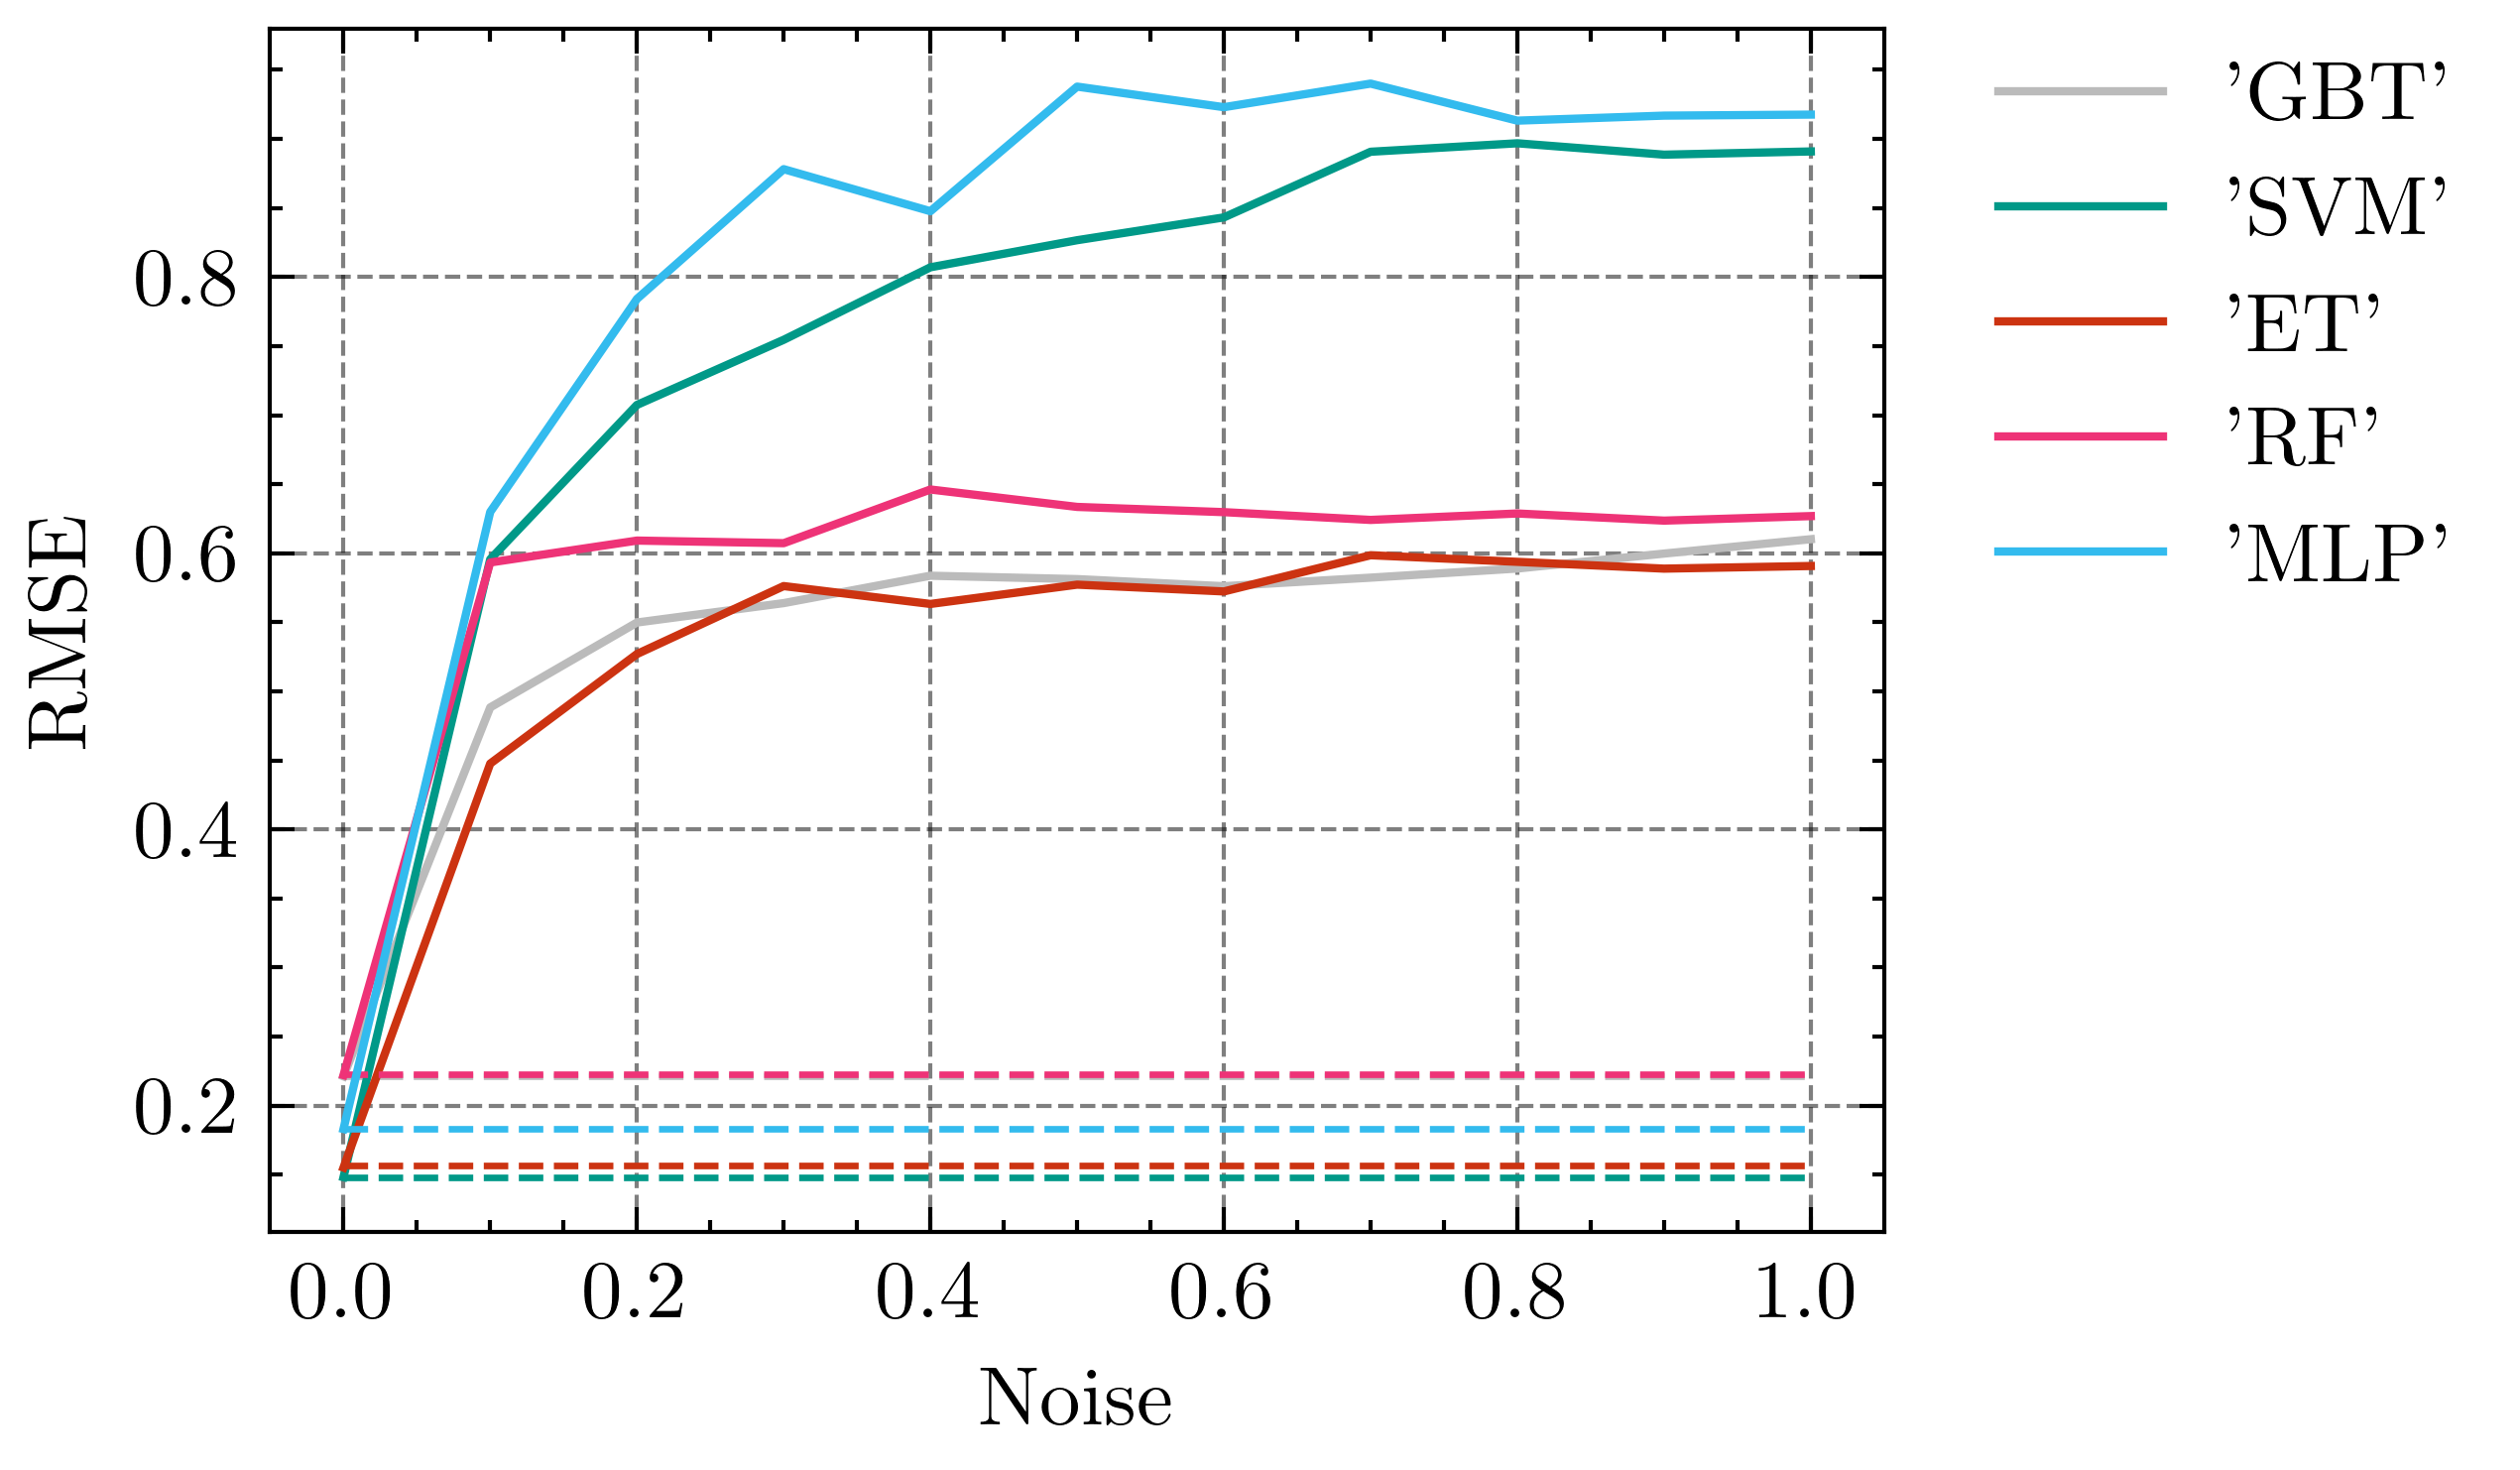
\includegraphics[width=0.9\textwidth]{chap5/images/results_noise}
    \end{tcolorbox}
    \caption{Comparison of performance on noisy data.
    The x-axis shows how many percent of the noisy dataset where added to the training data.
    The y-axis shows the RMSE metric.
    The dotted lines show the default performance of the model.
    The solid lines show the performance of the model when noise was added to the training data.
    }
    \label{fig:results-noise-fig}
\end{figure}

Comparing the noise test with the missing value test it can be seen that they yield quite different results.
In the missing values test the \ac{MLP} and \ac{SVM} models performed the best while the opposite is true when noise
was added to the training data.
With added noise all tree-based learning algorithms perform better.
Since the difference between all models in the missing values test wasn't that big the noise test could be
prioritised for the model selection but this will be discussed further in
~\cref{subsec:how-to-apply-the-results-in-practise}


\section{DP4: Stability}\label{sec:stability}
To evaluate the stability of the models, the \ac{LOOCV} can be used.
LOOCV is a type of Cross-Validation in which one sample is used for validation and the remaining data is used for
training
~\cite[p. 200--201]{gareth2013introduction}.
To evaluate the model's stability, the \ac{LOOCV} was repeated for all samples in the dataset, resulting in a total
of $n$ iterations.
The stability of the model was then determined by calculating the average prediction error across all iterations,
using the equation provided in \cref{eq:loocv}~\cite[p. 201]{gareth2013introduction}.

\begin{tcolorbox}[arc=0pt,boxrule=0.5pt]
    \begin{equation}
        CV_{(n)} = \frac{1}{n} \sum_{i=1}^{n} \text{MSE}_{i}\label{eq:loocv}
    \end{equation}
\end{tcolorbox}

The default metric for \ac{LOOCV} is usually the MSE, in this case the RMSE does not provide any additional
information since it is only the square root of the MSE.
Additionally the resulting \ac{MSE} is a poor estimate of the model's
generalization error since only one sample is used for validation.
But the goal of this section is to evaluate the stability of the model and not the generalization error.
The final stability is determined by the standard deviation of the Cross-Validation scores
~\cite[p. 201]{gareth2013introduction}.
A low standard deviation across all folds indicates that the model can generate consistent results when trained on
different datasets, which suggests a more stable model.

It is worth mentioning that there are numerous methods for determining a model's stability.
In this study \ac{LOOCV} was chosen for several reasons:
First, \ac{LOOCV} uses almost all the available data for training.
Since the dataset used in this study is relatively small, using all the data for training is advantageous.
Second, \ac{LOOCV} typically has lower bias due to the larger training set.
Lastly, various approaches were attempted to measure the model's stability and \ac{LOOCV} delivered
the most stable and interpretable results.
The primary drawback of this method is its computational expense since it
requires $n$ iterations.

The \cref{subsec:results-stability} presents the mean Cross-Validation score and standard deviation for each model.
The focus of the analysis is on the standard deviation since it provides a better indication of the model's stability.
As mentioned earlier, the \ac{CV} score using \ac{LOOCV} is a poor estimator of the model's generalization error.

\subsection{Results}\label{subsec:results-stability}

The \cref{tab:results-stability} shows the mean cross-validation score and standard deviation for each model.
In order to evaluate the stability of the model, the standard deviation was used as the primary metric.
The stability analysis reveals that the Gradient Boosting model is the most stable with a standard
deviation of 0.183.
The Extra Trees and Random Forest model exhibit similar levels of stability with mean CV score of 0.047 and 0.049,
and standard deviations of 0.206 and 0.194
It can be observed again, similar to the evaluation of the robustness that the MLP and SVM models exhibit
lower stability levels compared to the other models even though they where the most promising in the evaluation of
the correctness.

While stability is an important factor to consider, other aspects in particular the generalization error (correctness)
should be also taken into account.

\begin{table}[h]
    \begin{tcolorbox}[arc=0pt,boxrule=0.5pt]
% \sisetup{group-minimum-digits = 4}
        \centering
        \begin{tabular}{ll}
            \toprule
            \thead{\textbf{Model Name}} & \thead{\textbf{mean cv score ± std}}
            \\
            \toprule
            \textbf{Gradient Boosting}      & 0.038 ± 0.183 \\
            \hdashline
            \textbf{Random Forest}          & 0.047 ± 0.206 \\
            \hdashline
            \textbf{Extra Trees}            & 0.049 ± 0.194 \\
            \hdashline
            \textbf{Support Vector Machine} & 0.053 ± 0.244 \\
            \hdashline
            \textbf{MLP}                    & 0.053 ± 0.244 \\
            \hdashline
            \bottomrule
        \end{tabular}
    \end{tcolorbox}
    \caption{Results of the stability analysis. Sorted in ascending order by the standard deviation.}
    \label{tab:results-stability}
\end{table}

The \ac{DP}s 1 to 4 evaluated mostly the performance of the models. The next \ac{DP} will focus on the questions how
much resources are needed to train and use the models.


\section{DP5: Resource utilization}\label{sec:resource-utilization}

To evaluate the resource utilization, several metrics can be employed.
As discussed in \cref{subsec:dp5-resource-utilization}, this study focuses on time, computational power,
and memory resources.
Consequently, the metrics utilized to assess resource utilization include training time, inference time, and memory
usage.

The training time is measured in milliseconds and refers to the time that is required to train the model.
Training a model needs computational resources such as memory and CPU power, thus the longer the training process
takes the more resources are needed.
Therefore a shorter training time is preferred.
To measure the training time the python function \texttt{time.time} is employed.
The function does return the time in milliseconds since the epoch.
The time is recorded before and after the model is fitted and the difference between the two values
represents the training time.

The inference time is measured in milliseconds and refers to the time the models need to make predictions.
This metric is important for real-world use cases because users do not want to wait long for predictions and the
process also needs computational resources.
Since most models are able to make one prediction quite fast the inference time is measured for 100 predictions
using the \texttt{time.time} function again.

The memory usage is measured in megabytes (MB) and refers to the amount of memory that is required to run and save
the model.
A smaller memory footprint is preferred because it required less resources in the form of storage space.
To measure the memory usage the \texttt{memory\_usage} function from the package \texttt{memory\_profiler} is
employed.


\subsection*{Results}

The \cref{tab:results_resource_utilization} shows the results for the tests that where made.
Looking at the training time the Extra Trees and Random Forest models have the shortest training times
of 19.541 and 24.912 ms.
The Support Vector Machine and Gradient boosted models have intermediate training times.
The MLP is clearly the slowest with over 16 seconds.
The training time can be attributed the nature of the models and their training algorithm.
The RF and ET both benefit from the bagging technique which means that they training an ensemble of decision trees and
combine them to one big model.
This can be done in parallel and therefore massively speeds up the training
process (see \ref{subsubsec:random-forests}).
On the other side MLPs are typically more computational expensive since feeding forward and backpropagating the data
is not parallelizable and computationally expensive in general (see \cref{subsec:neural-networks}).

A comparable picture can be derived for the inference time.
This time the GBR, which is also a tree based algorithm is the fasted to make predictions while the MLP is the slowest.
The ET, RF and SVM models have comparable times.

Looking at the memory the MLP is using the most memory with 170 KB.
The other models have quite similar memory usage ranging from 157 to 158 KB.
Overall the memory space seems not to be a big issue for the models, a reason for that is the fact that the
dataset is not very big and the resulting models are also less complex.


\begin{table}[h]
    \begin{tcolorbox}[arc=0pt,boxrule=0.5pt]
        \centering
        \begin{tabular}{llll}
            \toprule
            \thead{\textbf{Model Name}} & {\thead{\textbf{Training time} \\
            \unit[]{ms}}}
            & {\thead{\textbf{Inference time} \\ \unit[]{ms}}} &
                {\thead{\textbf{Memory Usage} \\
            \unit{kb}}}
            \\
            \toprule
            \textbf{ET}  & 19541    & 1.939  & 157.93 \\
            \hdashline
            \textbf{RF} & 24912    & 2.027  & 157.684 \\
            \hdashline
            \textbf{GBR} & 43688   & 1.302  & 158.121 \\
            \hdashline
            \textbf{SVM} & 421007 & 2.587 & 158.082 \\
            \hdashline
            \textbf{MLP} & 16466261 & 17.988 & 170.715 \\
            \bottomrule
        \end{tabular}
    \end{tcolorbox}
    \caption{Results of the resource utilization analysis.}
    \label{tab:results_resource_utilization}
\end{table}


\section{DP6: Interpretability}\label{sec:interpretability}
In accordance with the definitions of interpretability outlined in \cref{sec:objectives-of-a-solution}, it
becomes apparent that quantitatively measuring interpretability is not viable.
However, alternative approaches can be employed to evaluate a model's interpretability.

%\cite{molnar2020interpretable} distinguishes between model-specific and model-agnostic approaches.
%Model-specific procedures are particular to one model, but model-agnostic methods can be applied to any model.
%~\cite[p. 19]{molnar2020interpretable}.

One strategy for achieving interpretability is restricting the selection of algorithms to those that yield
model specific interpretable outcomes.
Linear Regression models are one of good interpretable models~\cite[p. 17]{hall2019introduction}
Algoritms used in this study that are considered interpretable are Linear Regression
~\cite[p. 17]{hall2019introduction} and
Decision Trees~\cite[p. 20]{hall2019introduction}.
Nonetheless, as discussed in \cref{sec:dp1:-correctness}, these algorithms do not demonstrate sufficient
performance to be deemed viable solutions for predicting spring back.
Consequently, this study cannot rely on model-specific interpretability methods and should instead utilize model
-agnostic methods for generating explanations.

Also~\cite{hall2019introduction} differentiates between global and local interpretability.
Global interpretability refers to the ability to understand the overall behavior of
the model, while local interpretability refers to the ability to understand the behavior of the
model for a specific instance~\cite[p. 19]{hall2019introduction}.

It does not make sense to apply model-agnostic method on all trained models, it makes more sense to
apply the methods on the best performing models.
In the other parts of the evaluation, the Random Forest, Support Vector Machine and Multi Layer Perceptron models
where under the best performing models and are therefore the models that are used in the following
sections.

\subsection{Global Model-Agnostic Methods}\label{subsec:global-model-agnostic-methods}
In the following section, global model-agnostic methods are applied to the trained machine learning models to
understand their overall behavior.

% TODO Source?
Two commonly used methods for analyzing the relationship between input features
and the target variable are Feature Dependence Plots (FDP) and Partial Dependence Plots (PDP).
FDP plots illustrate the relationship between a feature and the target variable.
By analyzing these plots, we can identify which features have the strongest impact on the model's
predictions, making it easier to prioritize and refine the feature selection.

In the case of \ac{MLP}, there is no built-in feature importance, as the importance of each feature is determined by
the weights assigned to the perceptron.
For \ac{SVM}, feature importance cannot be directly derived from the model
because the algorithm applies a hyperplane that separates the data.
The importance of a feature depends on the influence of the hyperplane, which is not easily measurable.
Consequently, feature importance cannot be plotted for
the two chosen models.
In contrast, other algorithms, such as \ac{RF}, have built-in feature importance that can
be utilized to analyze the model.


The \cref{fig:feature-importances-rf1} compares and visualizes the relative importance of the features used for
training the model.
The figure was created using the \texttt{feature\_importances} attribute of the \texttt{RandomForestRegressor}
model from the \texttt{scikit-learn} library.
The PDP plots provides insights into the relevance and interactions of the
features.
As illustrated, thickness is the most important feature, followed by distance and die opening.
This means that changes in thickness have the most significant impact on spring back, while variations in the other
two features
have a comparatively smaller influence on the outcome.
In terms of interactions, all features are relevant, indicating that each feature contributes unique information to
the model.
This could suggest that the features are not highly correlated with each other, as their interactions
could already be observed in the correlation matrix shown in Figure~\ref{fig:correlation_matrix}.
Consequently, removing one feature would result in a significant loss of information and, therefore, poorer
performance of the model.

\begin{figure}[h]
    \begin{tcolorbox}[arc=0pt,boxrule=0.5pt]
        \centering
        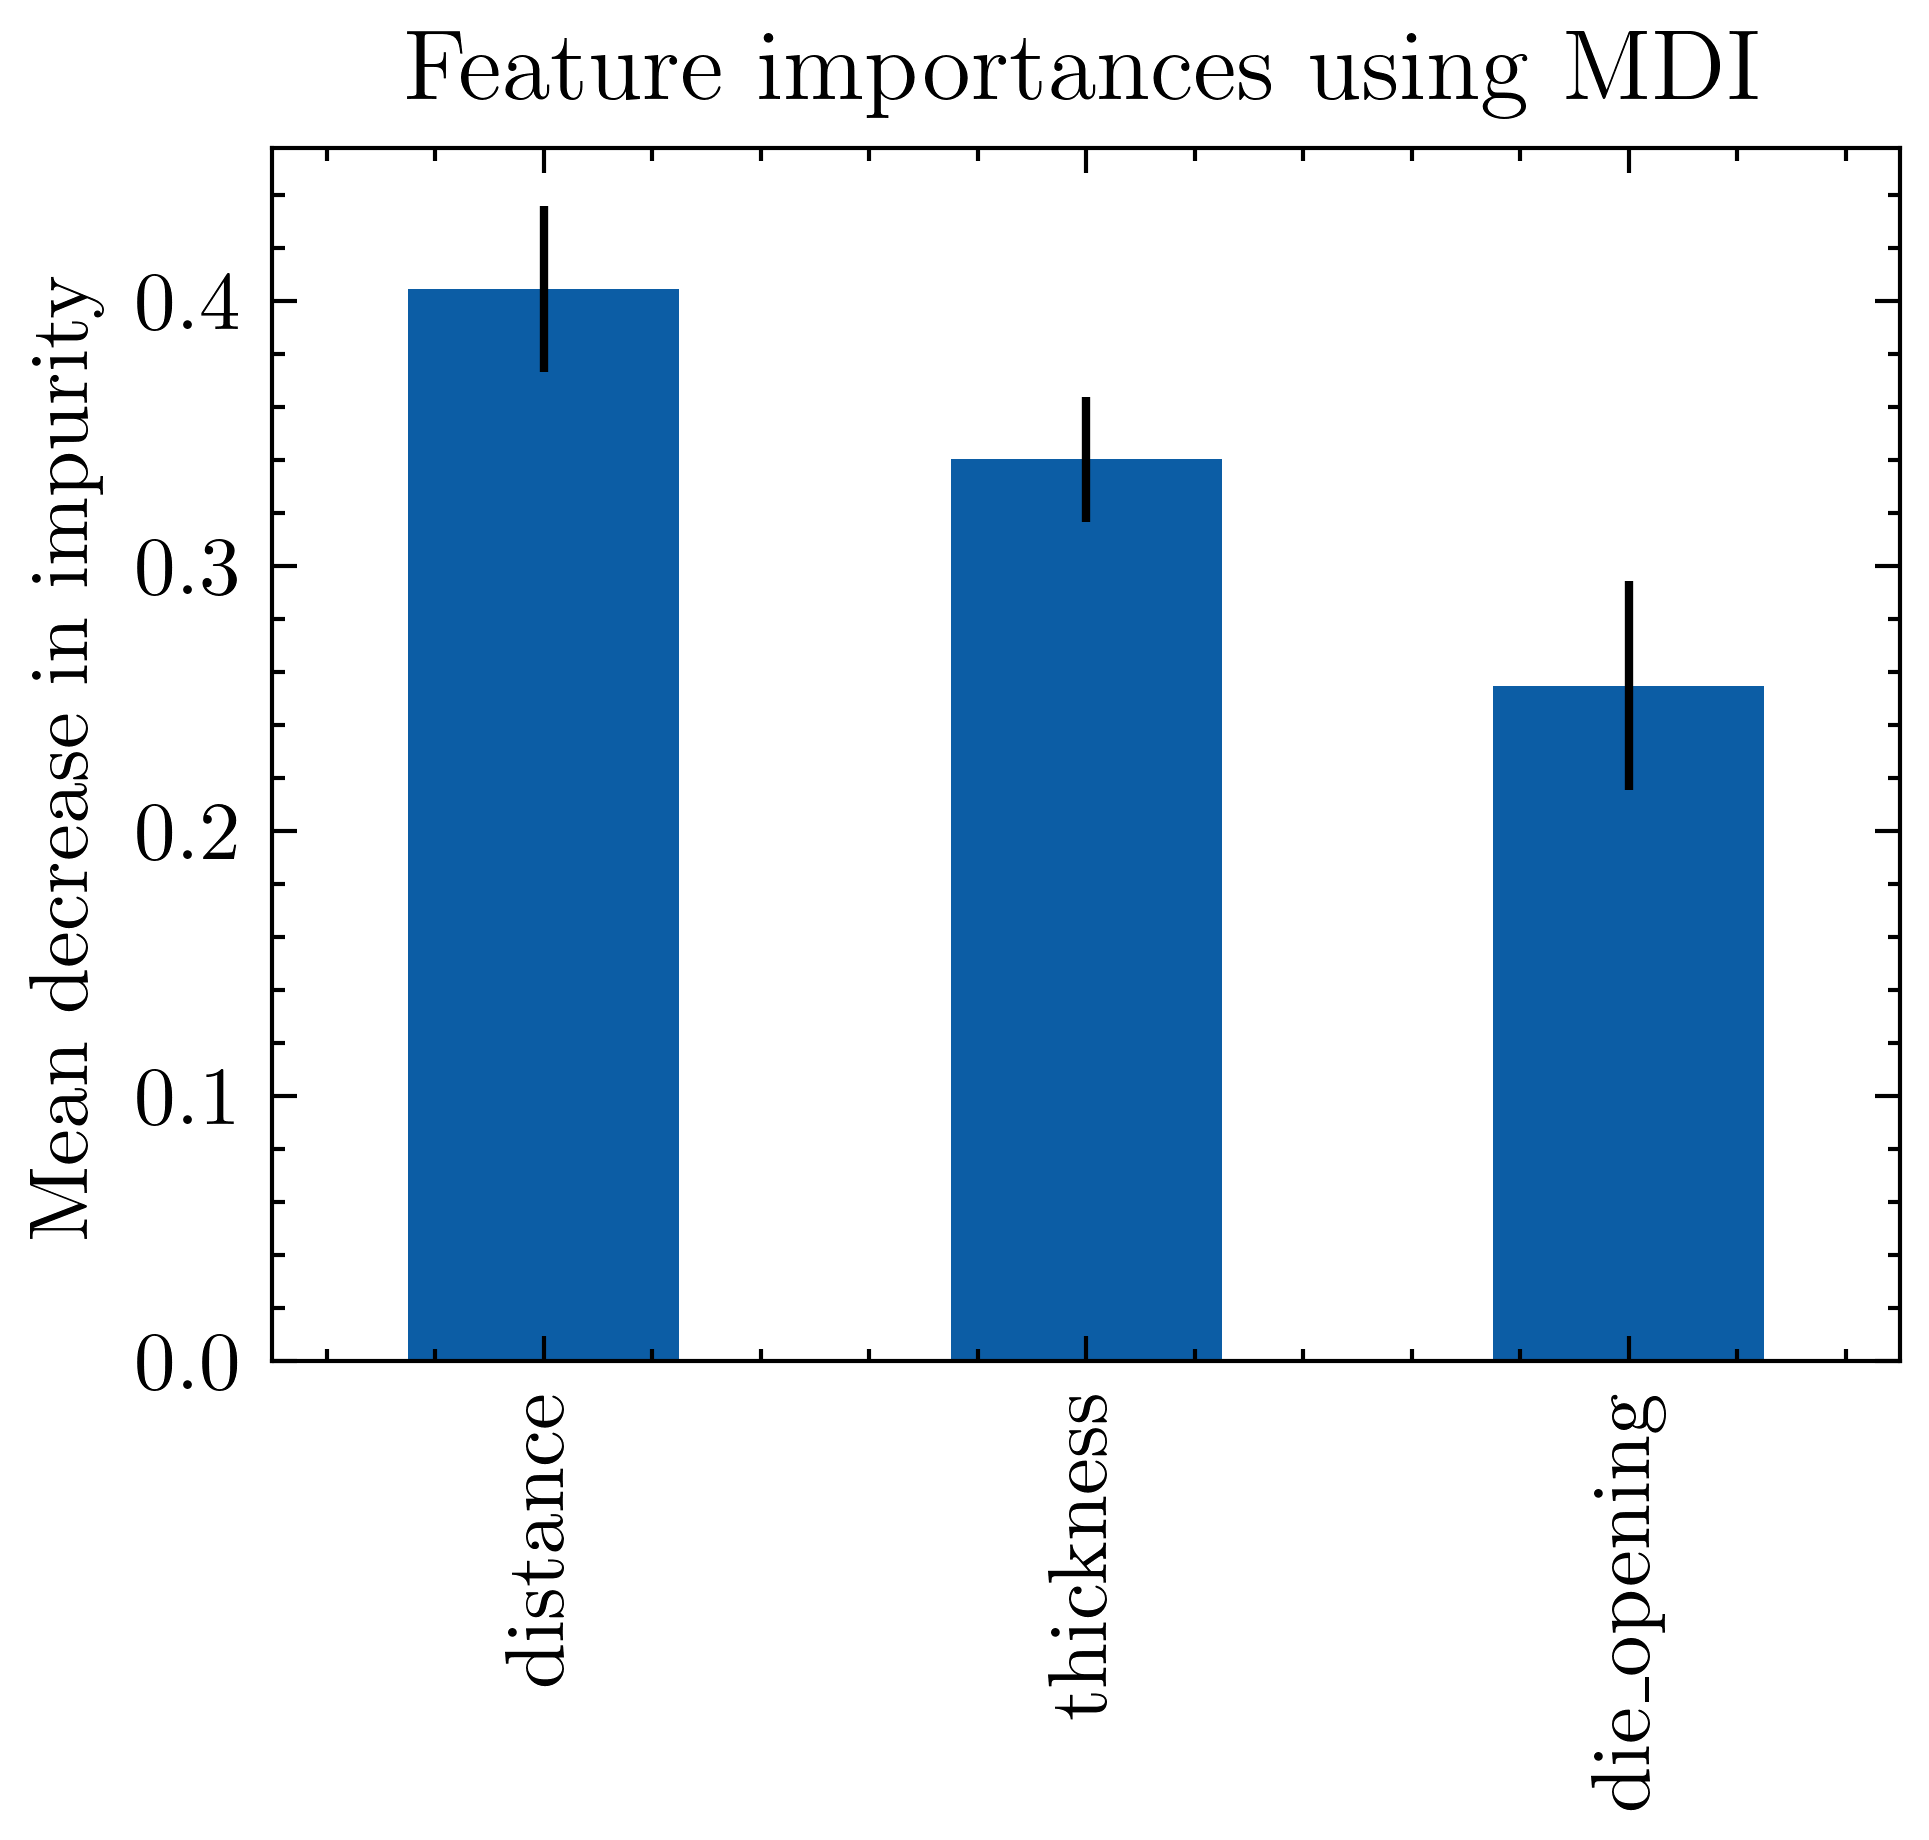
\includegraphics[width=0.5\textwidth]{chap5/images/rf_feature_importances}
    \end{tcolorbox}
    \caption{Feature importance of the random forest model.}
    \label{fig:feature-importances-rf1}
\end{figure}

The feature importance plot did facilitate a better understanding of the relationship between the features and the
target
variable.
However, they do not provide insights into exactly how the features influence the outcome.
PDP plots can be helpful for this purpose.

\subsection{Partial Dependence}
Another tool to measure the importance measure are PDP plots.
They measure the relationship between a target variable and a single predictor variable in a statistical model, while
keeping all other predictor variables constant
~\cite[pp. 313--314]{boehmke2019hands}.
A feature that exhibits a consistent partial dependence across all values is less important than a feature that
exhibits a non-linear relationship with the target variable.
While the feature importance plot shows the relative importance of each feature, the partial dependence plot shows
the impact of a single feature on the target variable.
\cite{scikit-learn} implementation of PDP plots is widely used and also utilized in this study.


In \cref{fig:partial_dependence_plots}, we can see the PDPs for two models: Support Vector Machines and
Multilayer Perceptron.
To the best knowledge of the author this is the first time that PDPs are used to analyze the relationship between
the input features and the target variable in the context of spring back prediction.

It can be seen that the plots for both models yield the same results for the three features.
The results show that a higher $y_p$ value leads to a greater spring back, while
increasing the thickness of the metal sheet results in a lower spring back.
The effect of the die opening is less significant than the other two features, but there is still a noticeable
increase in spring back with higher die opening.

The $y_p$ is the main factor that influences the bending angle and since most applications require a specific angle
this is not a viable option.
The results show that the most viable option to reduce the spring back in practical applications is to reduce the
thickness of the metal sheet.
As shown in \cref{fig:partial_dependence_plots}, especially for small thicknesses a change of 0.5 mm can lead to a
significant reduction of the spring back.
Since the same bending angle usually chan be achieved with multiple die openings it is also recommended to use a
smaller die opening to reduce the spring back as well.
The PDPs demonstrate that all features exhibit a non-linear relationship with the target variable.
This information can be useful for understanding the behavior of the models and the impact of different features on
the predicted outcome.


\begin{figure}
    \begin{tcolorbox}[arc=0pt,boxrule=0.5pt]
        \centering
        \subfigure[a]{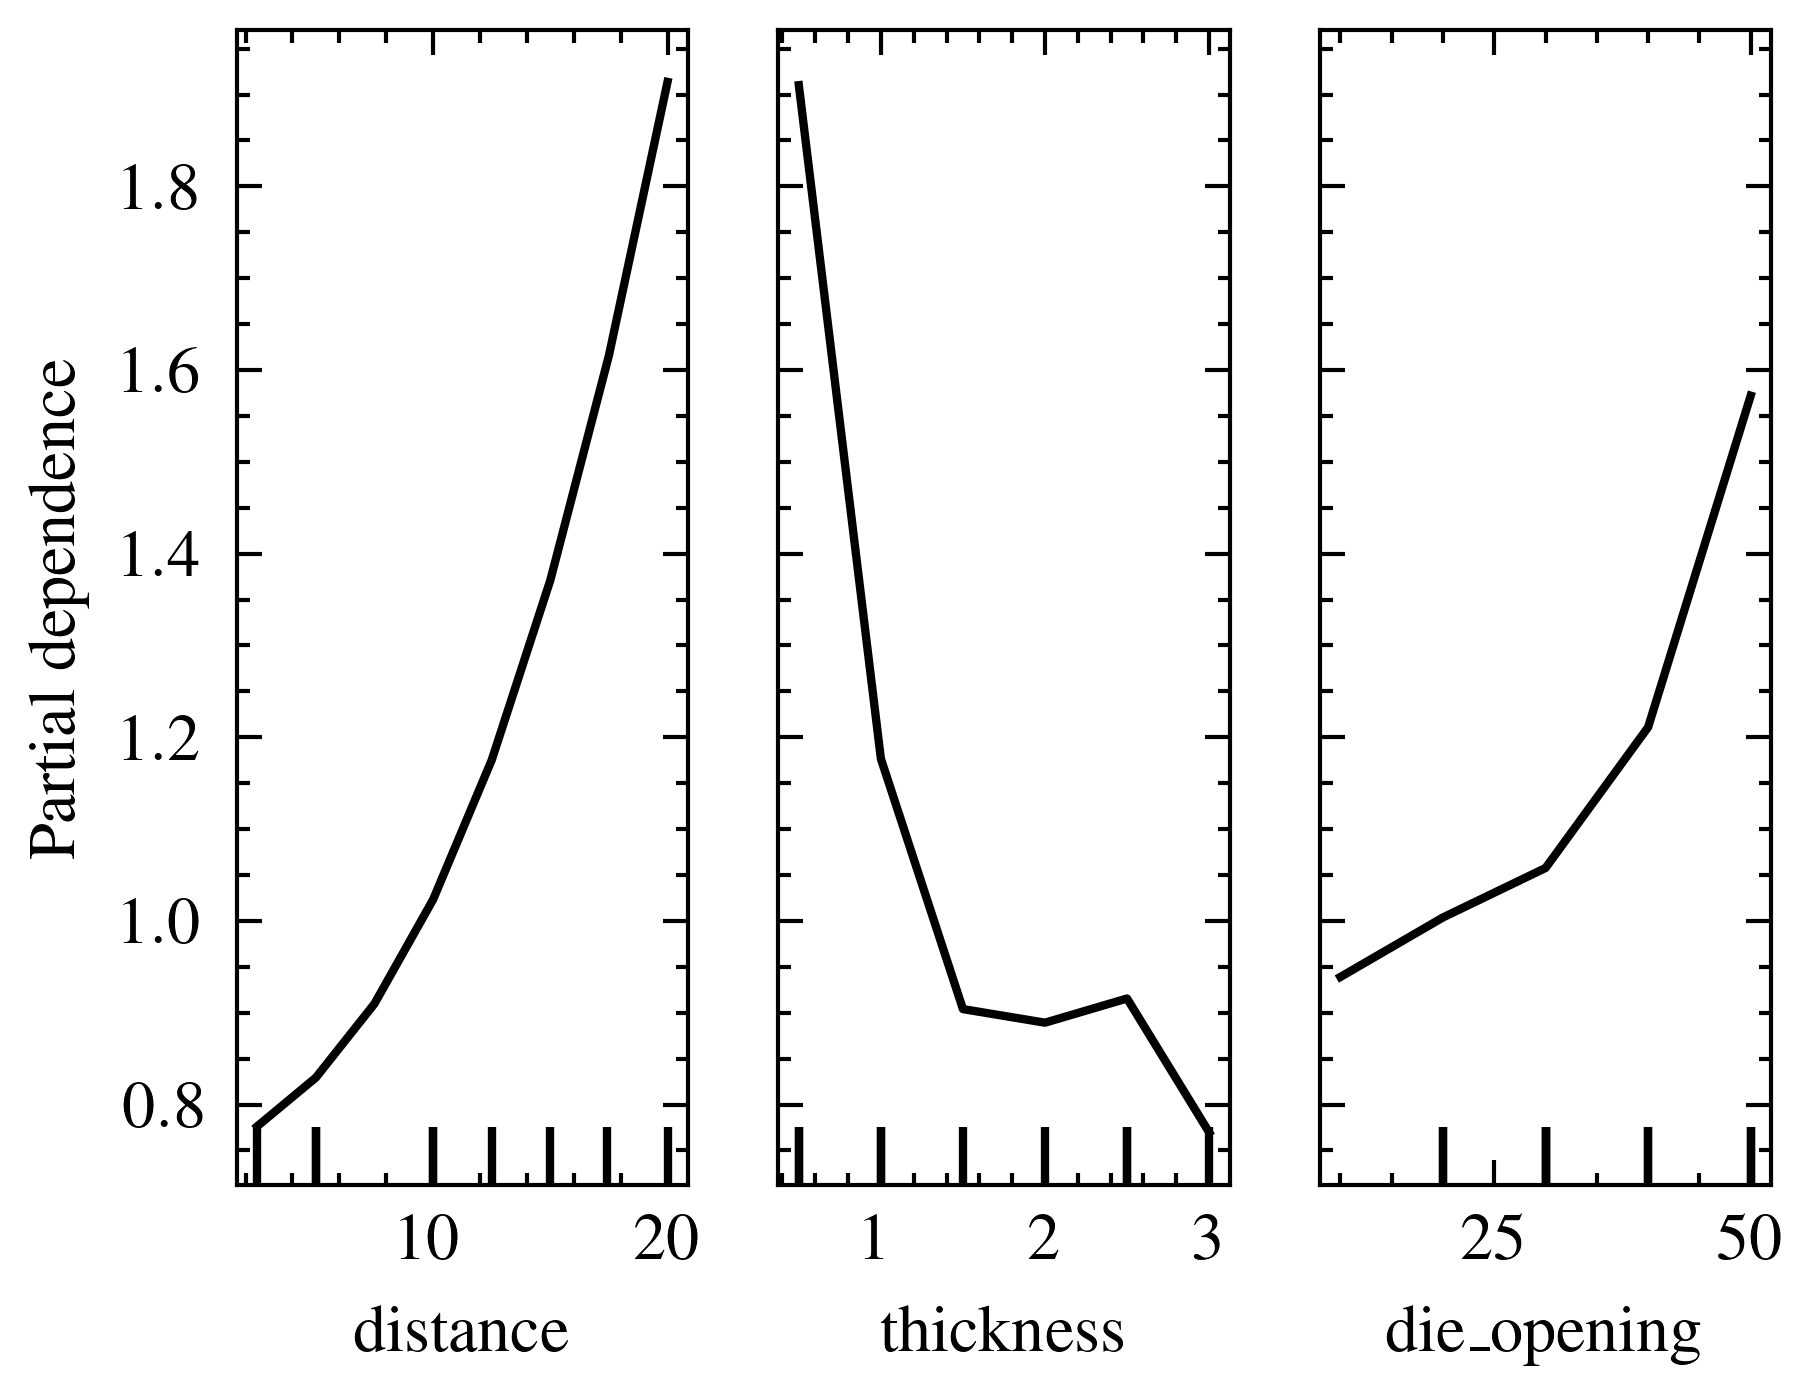
\includegraphics[width=0.4\textwidth]{chap5/images/partial_dependence_SVM}}
        \subfigure[b]{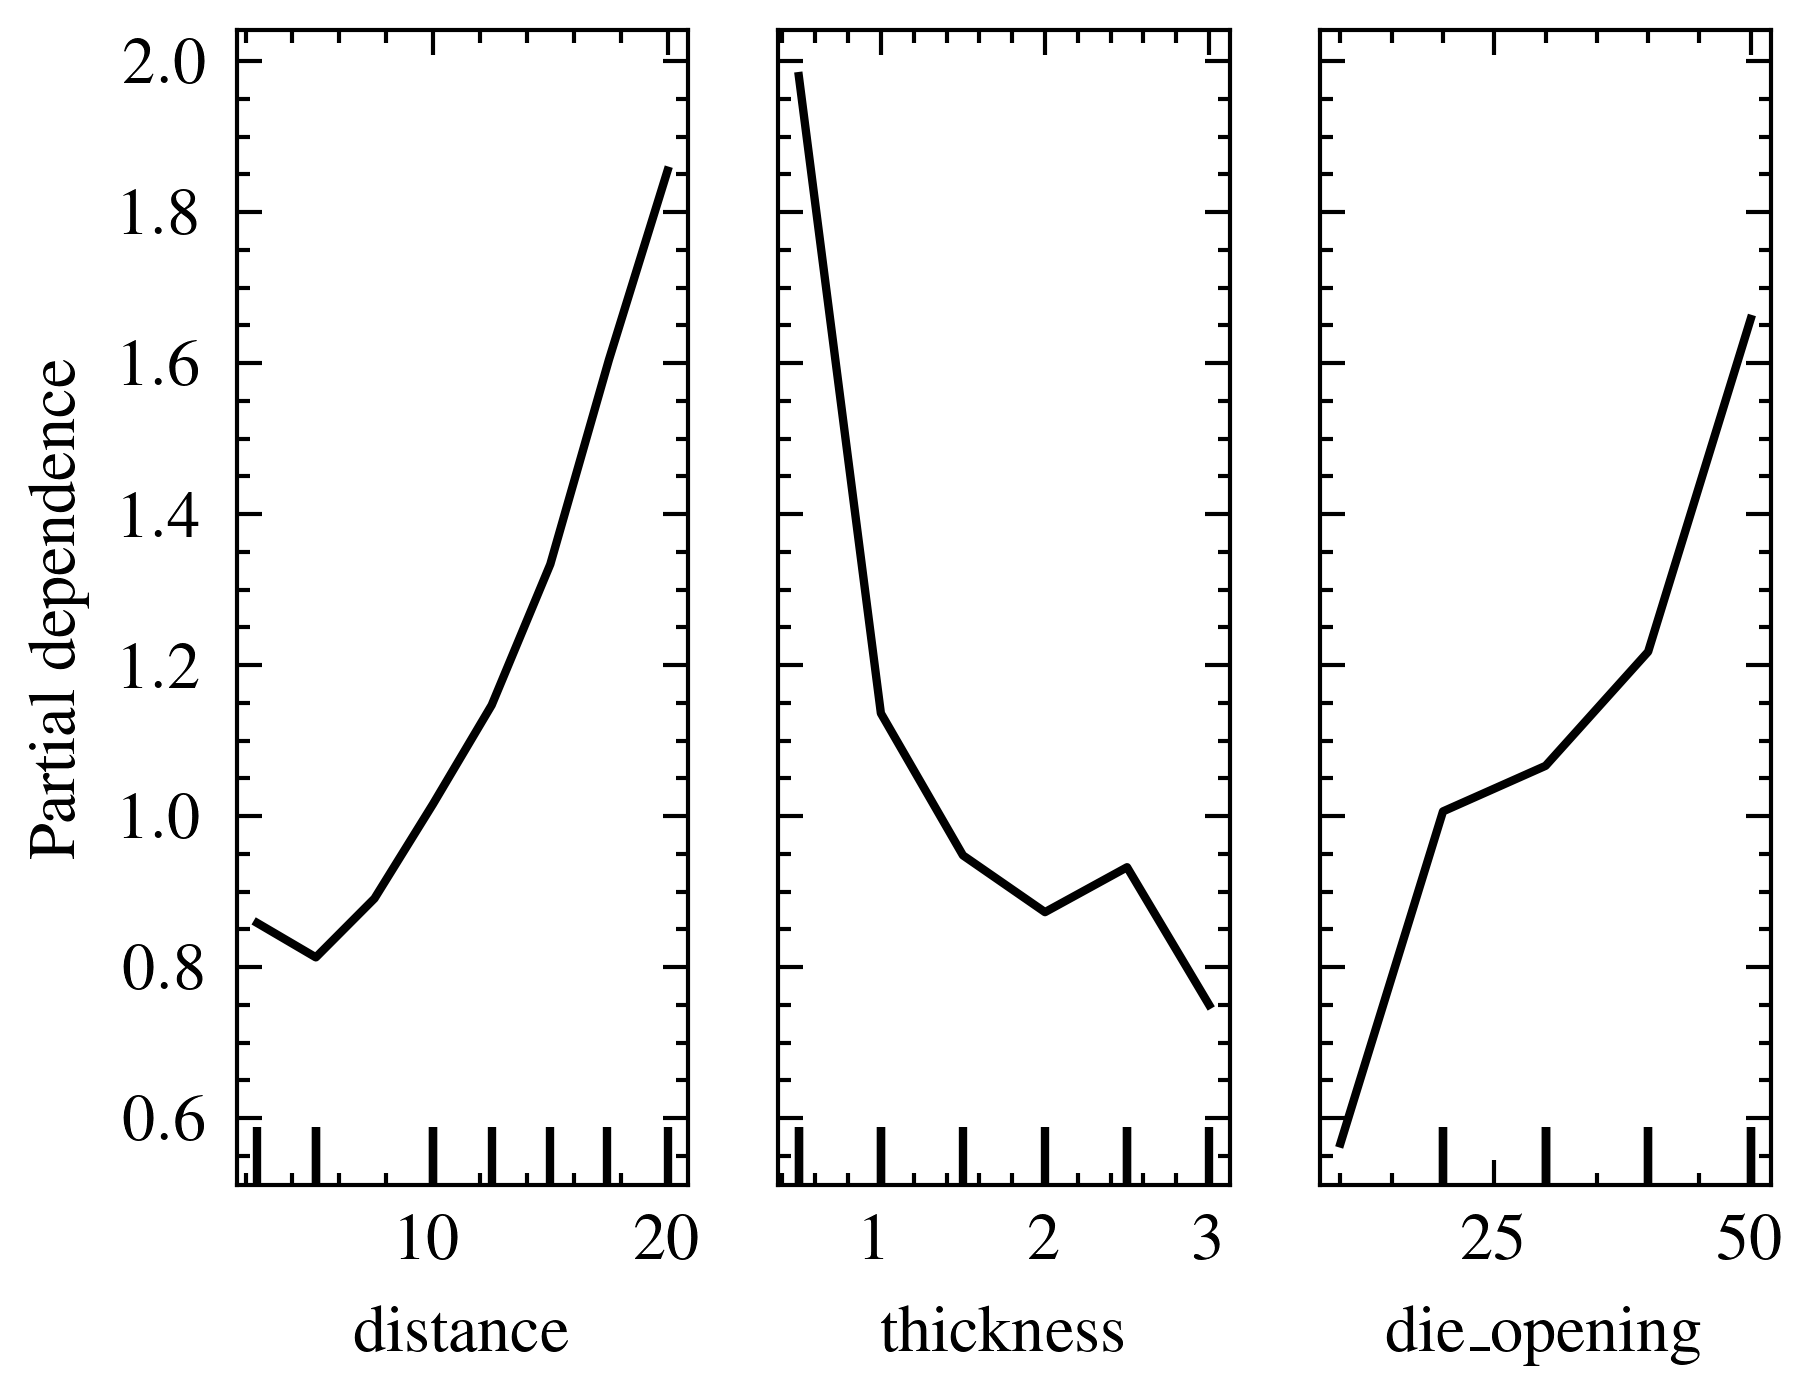
\includegraphics[width=0.4\textwidth]{chap5/images/partial_dependence_MLP}}
        \caption{DPD plots for [a] and SVM [b] MLP}
        \label{fig:partial_dependence_plots}
    \end{tcolorbox}
\end{figure}

%\begin{figure}[h]
%    \begin{tcolorbox}[arc=0pt,boxrule=0.5pt]
%        \centering
%        \begin{subfigure}{0.45\textwidth}
%            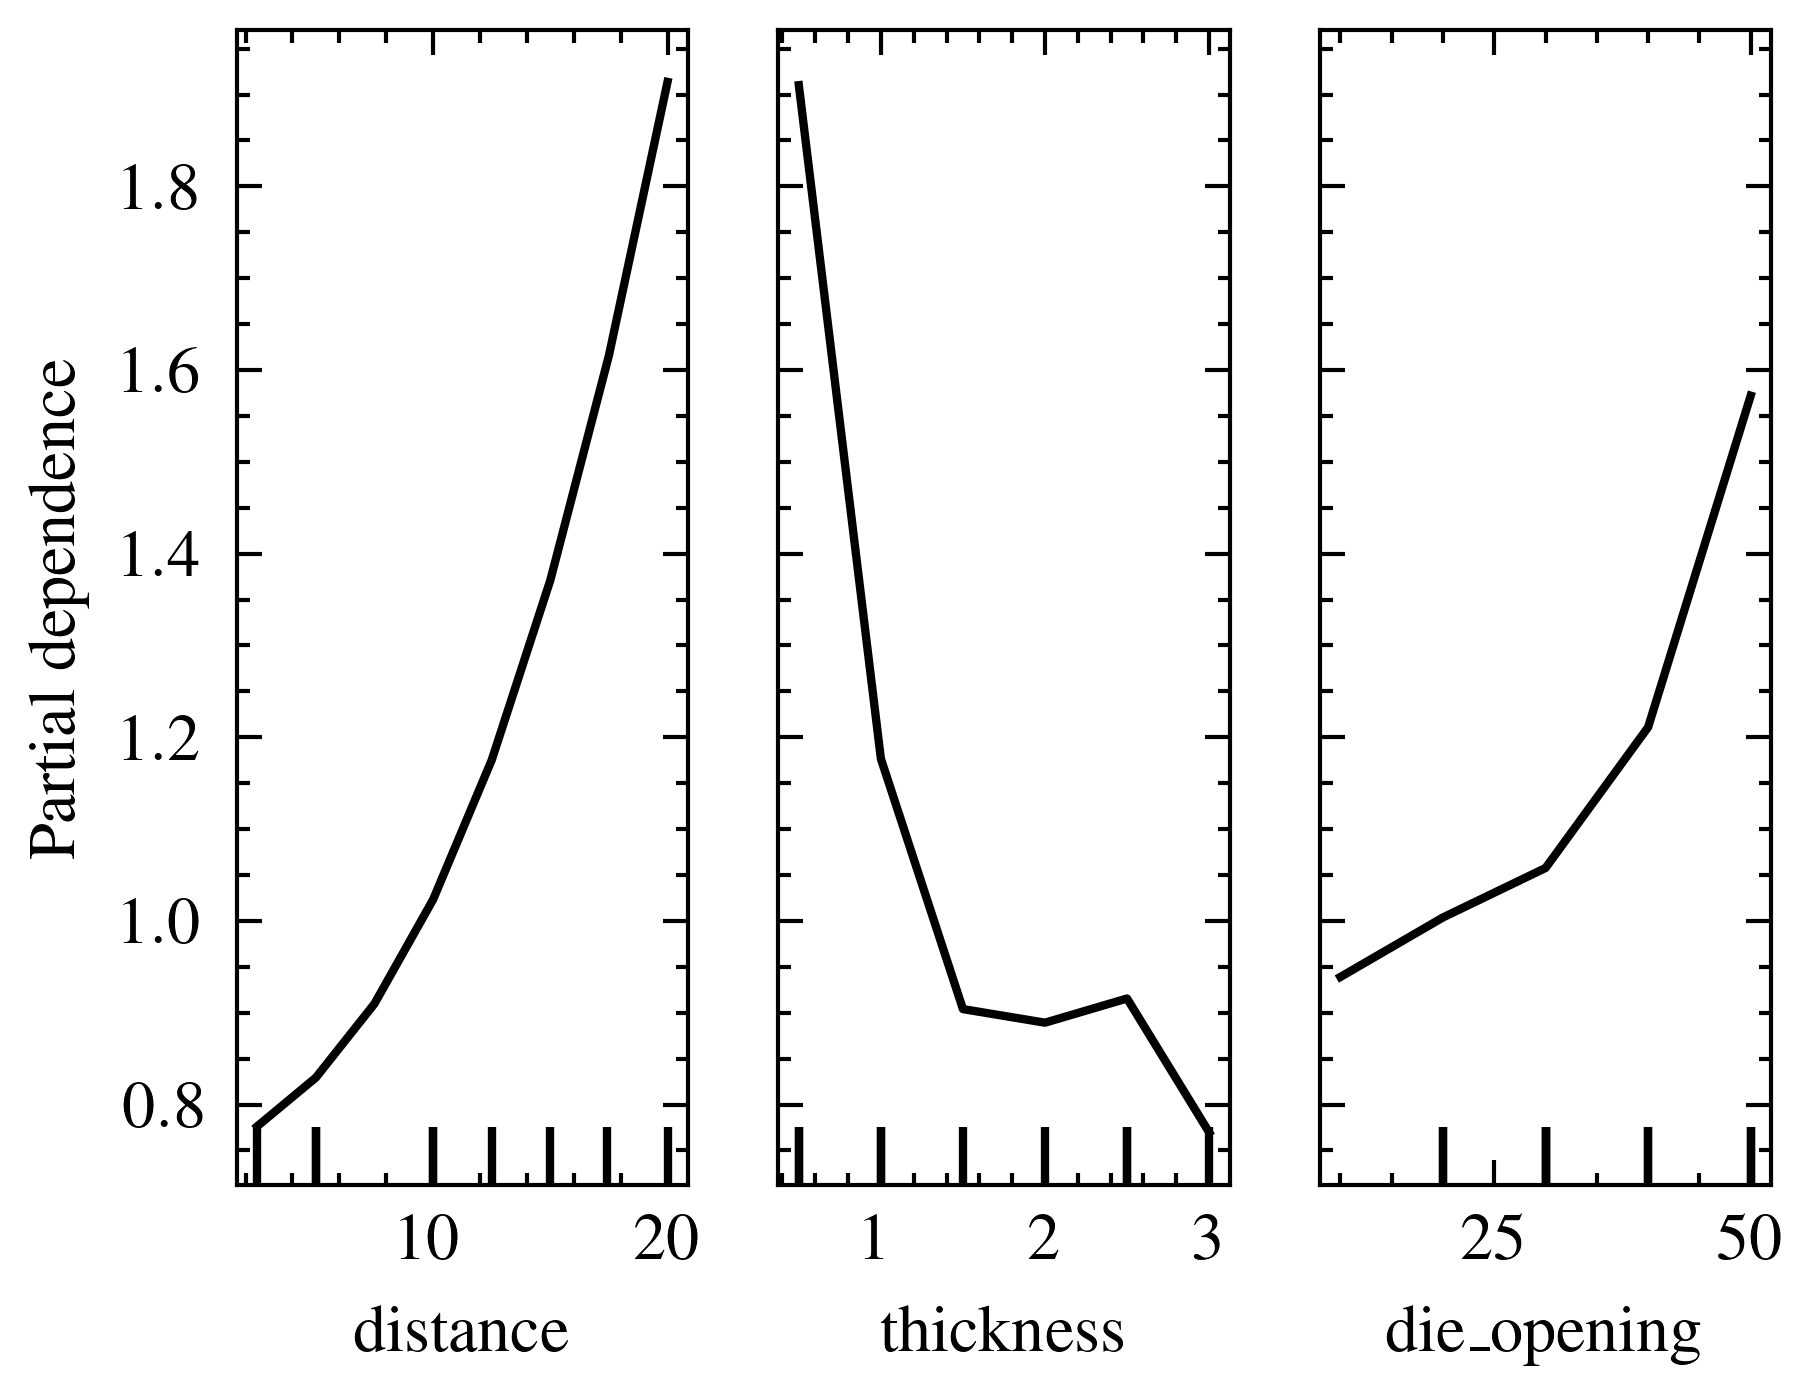
\includegraphics[width=\textwidth]{chap5/images/partial_dependence_SVM}
%            \caption{SVM}
%            \label{fig:feature_impoartances_rf}
%        \end{subfigure}
%        \hfill
%        \begin{subfigure}{0.45\textwidth}
%            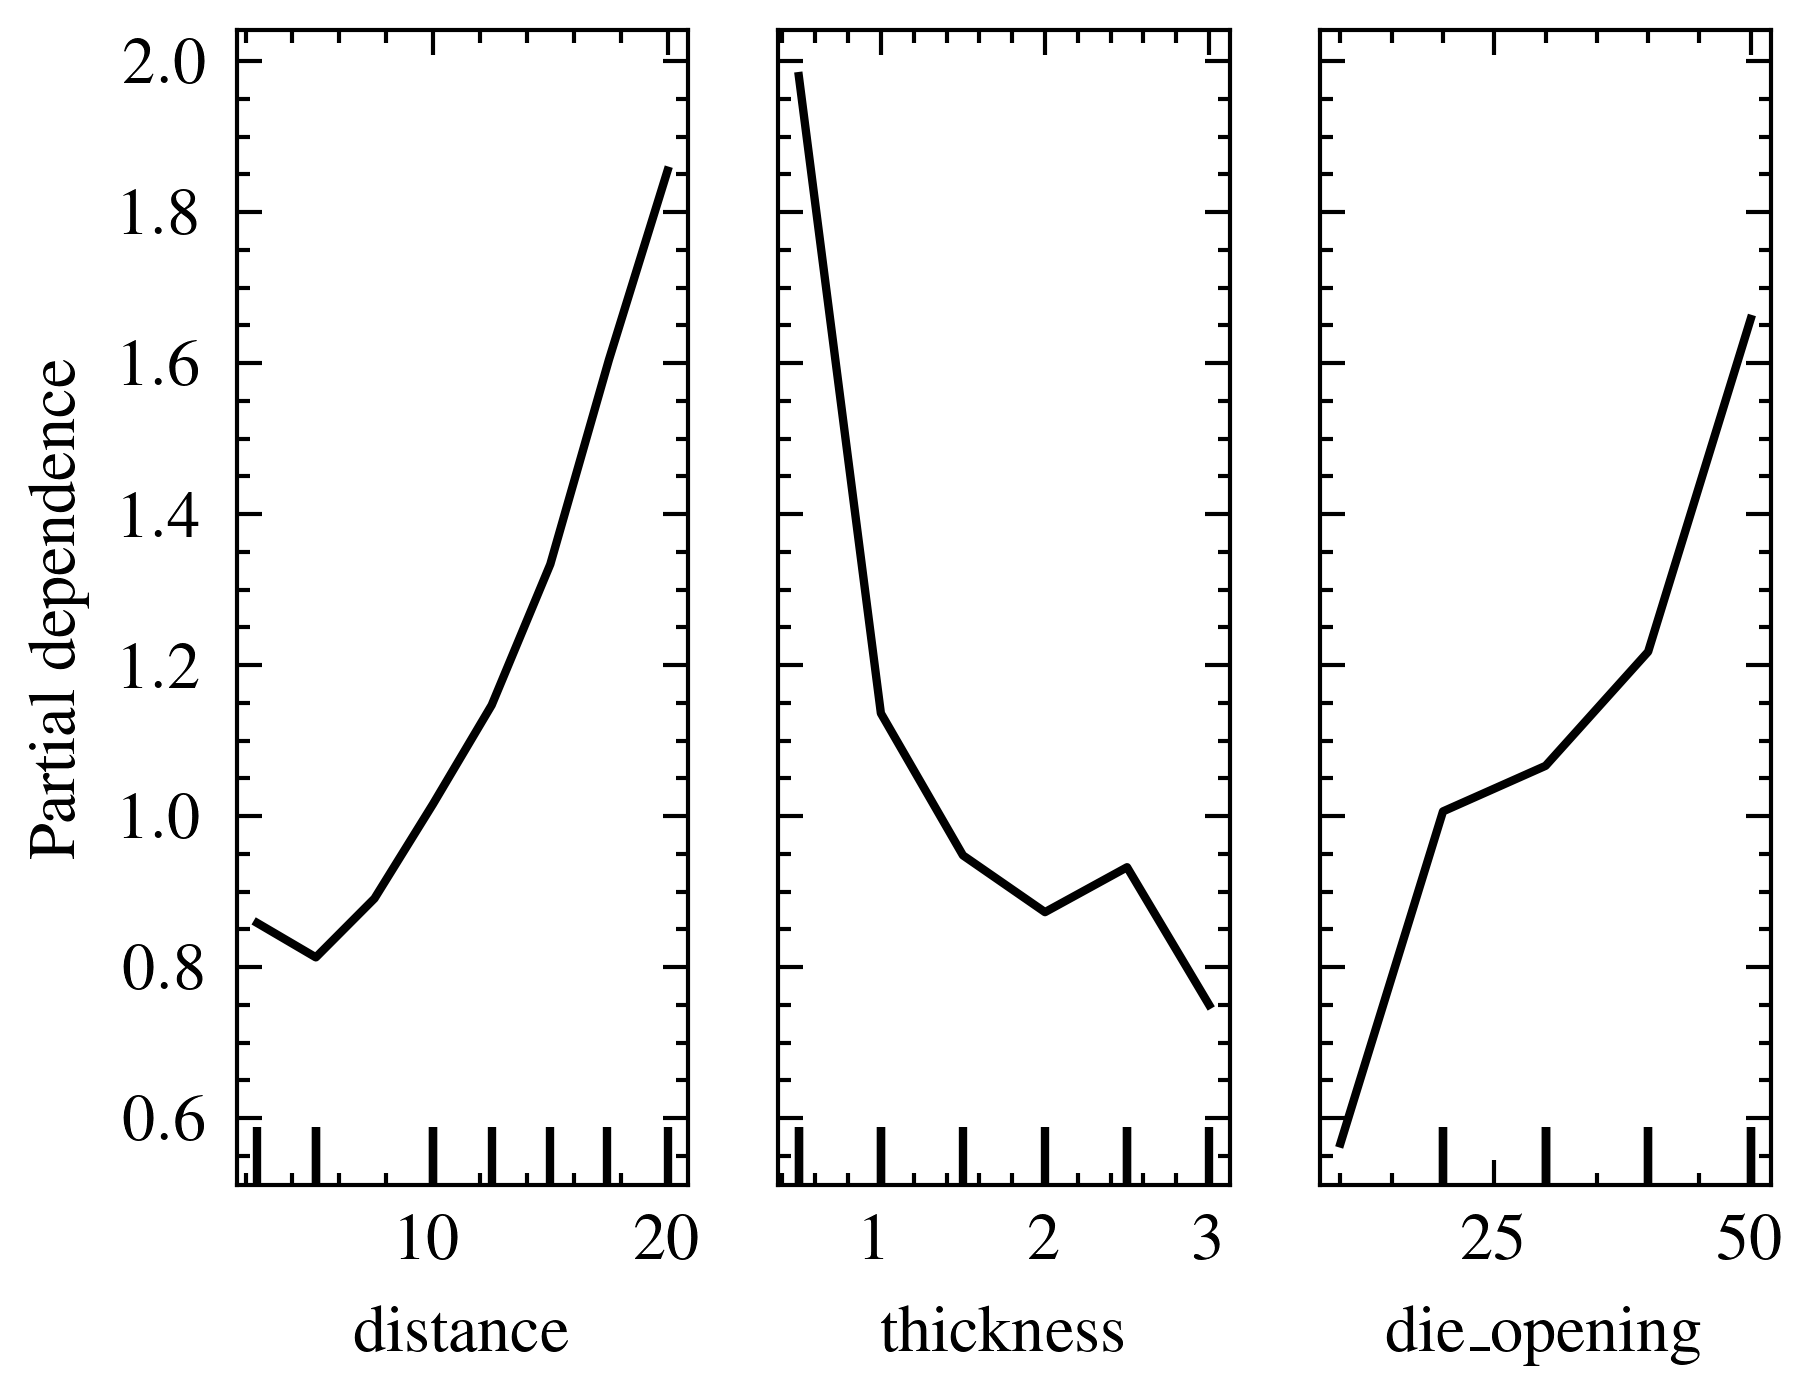
\includegraphics[width=\textwidth]{chap5/images/partial_dependence_MLP}
%            \caption{MLP}
%            \label{fig:partial_dependence_svm}
%        \end{subfigure}
%        \hfill
%    \end{tcolorbox}
%    \caption{Partial dependence plots generated with \textit{sci-kit learn}~\cite{scikit-learn}}
%    \label{fig:partial_dependence_plots}
%\end{figure}

It is important to note that partial dependence plots and feature importance plots are limited to
identifying linear relationships between features and the target variable.
Since this is not the case as state previously, the results of the partial dependence plots are
alternative models as permutation feature importance values are used to gain further
information.

\subsection{Permutation Feature Importance}\label{subsec:permutation-feature-importance-
and-shap}

PDP plots assess the impact on the model's prediction error when the values
of a feature a randomly permutes.
Permutation in this context means the process of randomly shuffling the values of a single features while keeping
the
values of all other features unchanged.
Thereby the association between the feature and the actual outcome is disrupted~\cite[]{scikit-learn}.
%~\cite[p. 157]{molnar2020interpretable}.
The importance of a feature is evaluated by assessing the degree to which permuting its values
results in an increase in the prediction error fo the model.
If permuting a features results in a significant increases in errors the features is deemed
important because the model relied on it for making accurate predictions.
Conversely, if permuting a feature doesn't change the prediction error is considered unimportant
because the model didn't utilize it for its prediction
~\cite[]{scikit-learn}.
%~\cite[p. 158]{molnar2020interpretable}.

The results for the MLP and SVM models presented in \cref{tab:permutation_feature_importance}.
The top section of the table shows the permutation importance of the feature for the $R^2$ while the bottom section
show the permutation importance for the $MSE$.
In this case again the $MSE$ was chosen since the original unit is not needed to interpret the table, therefore
$RMSE$
would not provide any additional information.
For each feature the permutation feature importance score as well as the standard derivation is listed.
If a feature achieves a higher permutation importance score it is considered to be more important, since it does
influence the outcome of the model more.
Additionally the standard derivation is given, a higher standard derivations suggest that the feature importance
score is more unstable.
For example the feature thickness has a permutation importance score of 1.337 with a standard derivation of
0.174.
Compared with the other feature this indicates that the feature thickness is the most important feature and
the standard derivation is relatively low, therefore the feature importance score is stable.

The results show that the MLP and the SVM models yield similar trends in the importance of features.
The features thickness and punch penetration have a high importance with their permutation causing a significant
increase in the prediction error both in $R^2$ and $MSE$.
This indicates that they are crucial for the decision making of the model.

What differs from the previous analysis: The die opening has a importance of zero in both models.
Ths implies does permuting this features does not have any influence on the prediction error.
This is a surprising result, that was to the best knowledge of the author not reported in previous research.
The result could be replicated with different models and different data sets, therefore it is not a random
occurrence.
There are two possible explanations for this:
\begin{enumerate}
    \item The die opening is not relevant for the decision making at all and does not provide any
    significant information.
    \item The die opening is important but only in combination with either the thickness or the
    penetration distance.
    This suggest that there might be an interaction effect that was not captured in previous analysis.
\end{enumerate}

Since the normal feature importance plots showed that die opening is important the second explanation is more
likely.
To further investigate this possibility a Partial Dependence Plot was created specifically for the die opening in
combination with either the thickness or the penetration distance.

\begin{table}[h]
    \begin{tcolorbox}[arc=0pt,boxrule=0.5pt]
        \centering
        \subfloat[Subtable 1 list of tables text][MLP]{
            \begin{tabular}{lll}
                \toprule
                \multicolumn{3}{}{\textbf{$R^2$}} \\
                \toprule
                thickness   & 1.337 & +/- 0.173542 \\
                \hdashline
                distance    & 1.293 & +/- 0.145488 \\
                \hdashline
                die opening & 0.000 & +/- 0.000000 \\
                \toprule
                \multicolumn{3}{l}{\textbf{$MSE$}} \\
                \toprule
                thickness   & 0.274 & +/- 0.035613 \\
                \hdashline
                distance    & 0.265 & +/- 0.029856 \\
                \hdashline
                die opening & 0.000 & +/- 0.000000 \\
                \bottomline
            \end{tabular}}
        \qquad
        \subfloat[Subtable 2 list of tables text][SVM]{
            \begin{tabular}{lll}
                \toprule
                \multicolumn{3}{}{\textbf{$R^2$}} \\
                \toprule
                distance    & 1.237 & +/- 0.139285 \\
                \hdashline
                thickness   & 1.178 & +/- 0.157247 \\
                \hdashline
                die opening & 0.000 & +/- 0.000000 \\
                \toprule
                \multicolumn{3}{l}{\textbf{$MSE$}} \\
                \toprule
                distance    & 0.254 & +/- 0.028583 \\
                \hdashline
                thickness   & 0.242 & +/- 0.032269 \\
                \hdashline
                die opening & 0.000 & +/- 0.000000 \\
                \bottomline
            \end{tabular}}
    \end{tcolorbox}
    \caption{Permutation feature importance}
    \label{tab:permutation_feature_importance}
\end{table}

To investigate the joint performance of the die opening feature with the other two features,
again partial dependence plots can be used.
The \cref{fig:dpd-distance-die-opening} shows a two-way partial dependence plot for the \ac{MLP} model.
It is segmented into three individual plots: The first two plots show the partial dependence of the distance and the
die opening.
But the most interesting is the third plot which the interaction of the two input features distance (x-axis) and die
opening (y-axis).
The slope of the contour lines indicates the direction of the effect of the die opening on the
prediction.
The contour lines are colored and labeled according to the value of the prediction.
It can be seen that the contour lines are not parallel which suggest the two features interact
with each other and therefore have a joint effect on the model prediction.

This means that the second explanation mentioned above is correct and the die opening is not irrelevant for the
model prediction but just interacts with the other two features.
Therefore it only affect the prediction in combination with the other two features.
To the best knowledge of the author this interaction was not yet reported in previous research and is a new
finding of this study.


\begin{figure}[h]
    \begin{tcolorbox}[arc=0pt,boxrule=0.5pt]
        \centering
        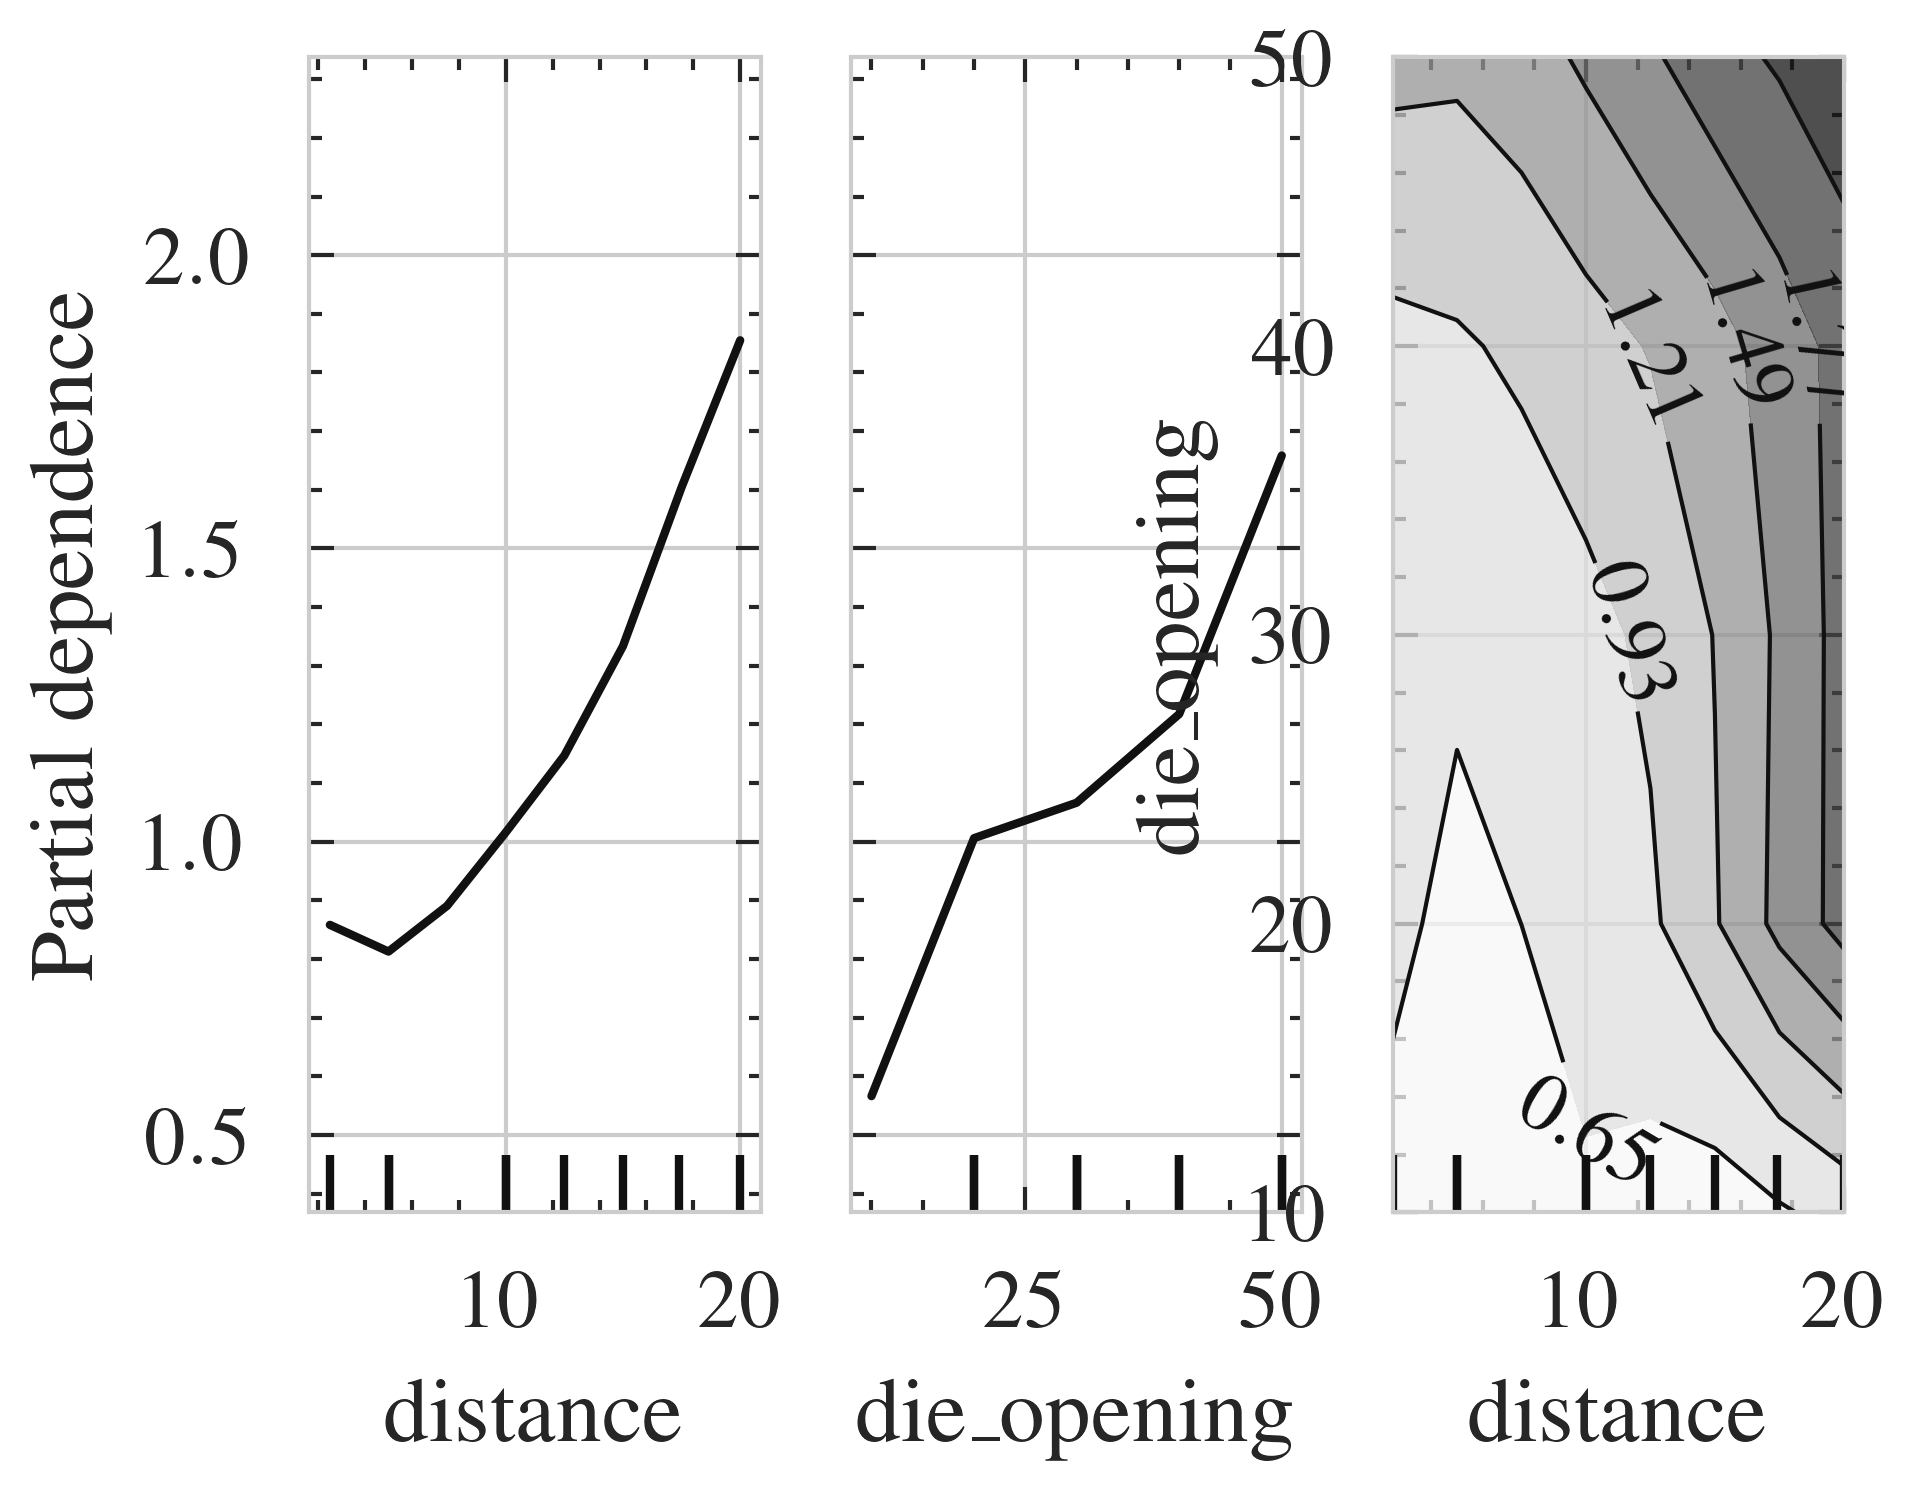
\includegraphics[width=0.6\textwidth]{chap5/images/pdp_distance_die_opening}
    \end{tcolorbox}
    \caption{DPD distance and die opening}
    \label{fig:dpd-distance-die-opening}
\end{figure}

\subsection{Local Model Agnostic Methods}\label{subsec:local-model-agnostic-methods}
Local interpretability refers to the ability to understand the behavior of the model for a
specific instance and is often used to explain the predictions of a model
~\cite[p. 19]{hall2019introduction}.
Model agnostic methods can be used to explain the predictions of any model types and not only specific algorithms
~\cite[p. 20]{hall2019introduction}.

Local methods rely on interpreting individual instances from a dataset and as such, it is
crucial to select representative samples.
One way to achieve this is by considering the V/t ratio of each instance.
The local model agnostic method LIME was applied on different machine learning models.
But it did not yield any meaningful results.
Therefore no further analysis on the local model agnostic methods was performed.

Concluding the previous sections, different method where used evaluate the models trained in this study.
The results will now be demonstrated in the next section.


\section{Demonstration}\label{sec:demonstration}
This section represents the demonstration activity in the \ac{DSR} process.
This activity focuses on the demonstration of the developed models in specific selected scenarios and not the
overall performance like in the evaluation activity.
For this purpose three scenarios are selected and and for each the models are demonstrated.

For the current dataset, the V/t ratios range from 10 to 100.
The highest ratio can be achieved by bending a 0.5 mm thin metal sheet using a 50 mm wide die opening, while the
lowest ratio is achieved by bending a 1 mm thick sheet on a 10 mm die opening.

According to~\cite{cruz2021application} the recommended V/t ratios in industrial practices are between 6 and
10~\cite[p. 7]{cruz2021application}.
These values could not be reproduced in the dataset used in this study, the lowest V/t ratio in the chosen experimental
setup is 10, below that it was not possible to squeeze metals larger than 1 mm through a die opening of 10 mm.
Upon examining \cref{fig:springback-heatmap}, it is evident that the recomended V/t ratios are higher for the
dataset used in this study.
Again it can be seen that a greater die opening and a reduced thickness results in a higher spring back.
Notably, the data points with a high V/t ratio like $t$ 0.5 $V$ 40 and $t$0.5 $V$ 50 exhibit particularly elevated
spring
backs relative to the remaining data set.
Conversely, all the data collected with a with a low V/t ratios have a lower spring back values.

\begin{figure}[h]
    \begin{tcolorbox}[arc=0pt,boxrule=0.5pt]
        \centering
        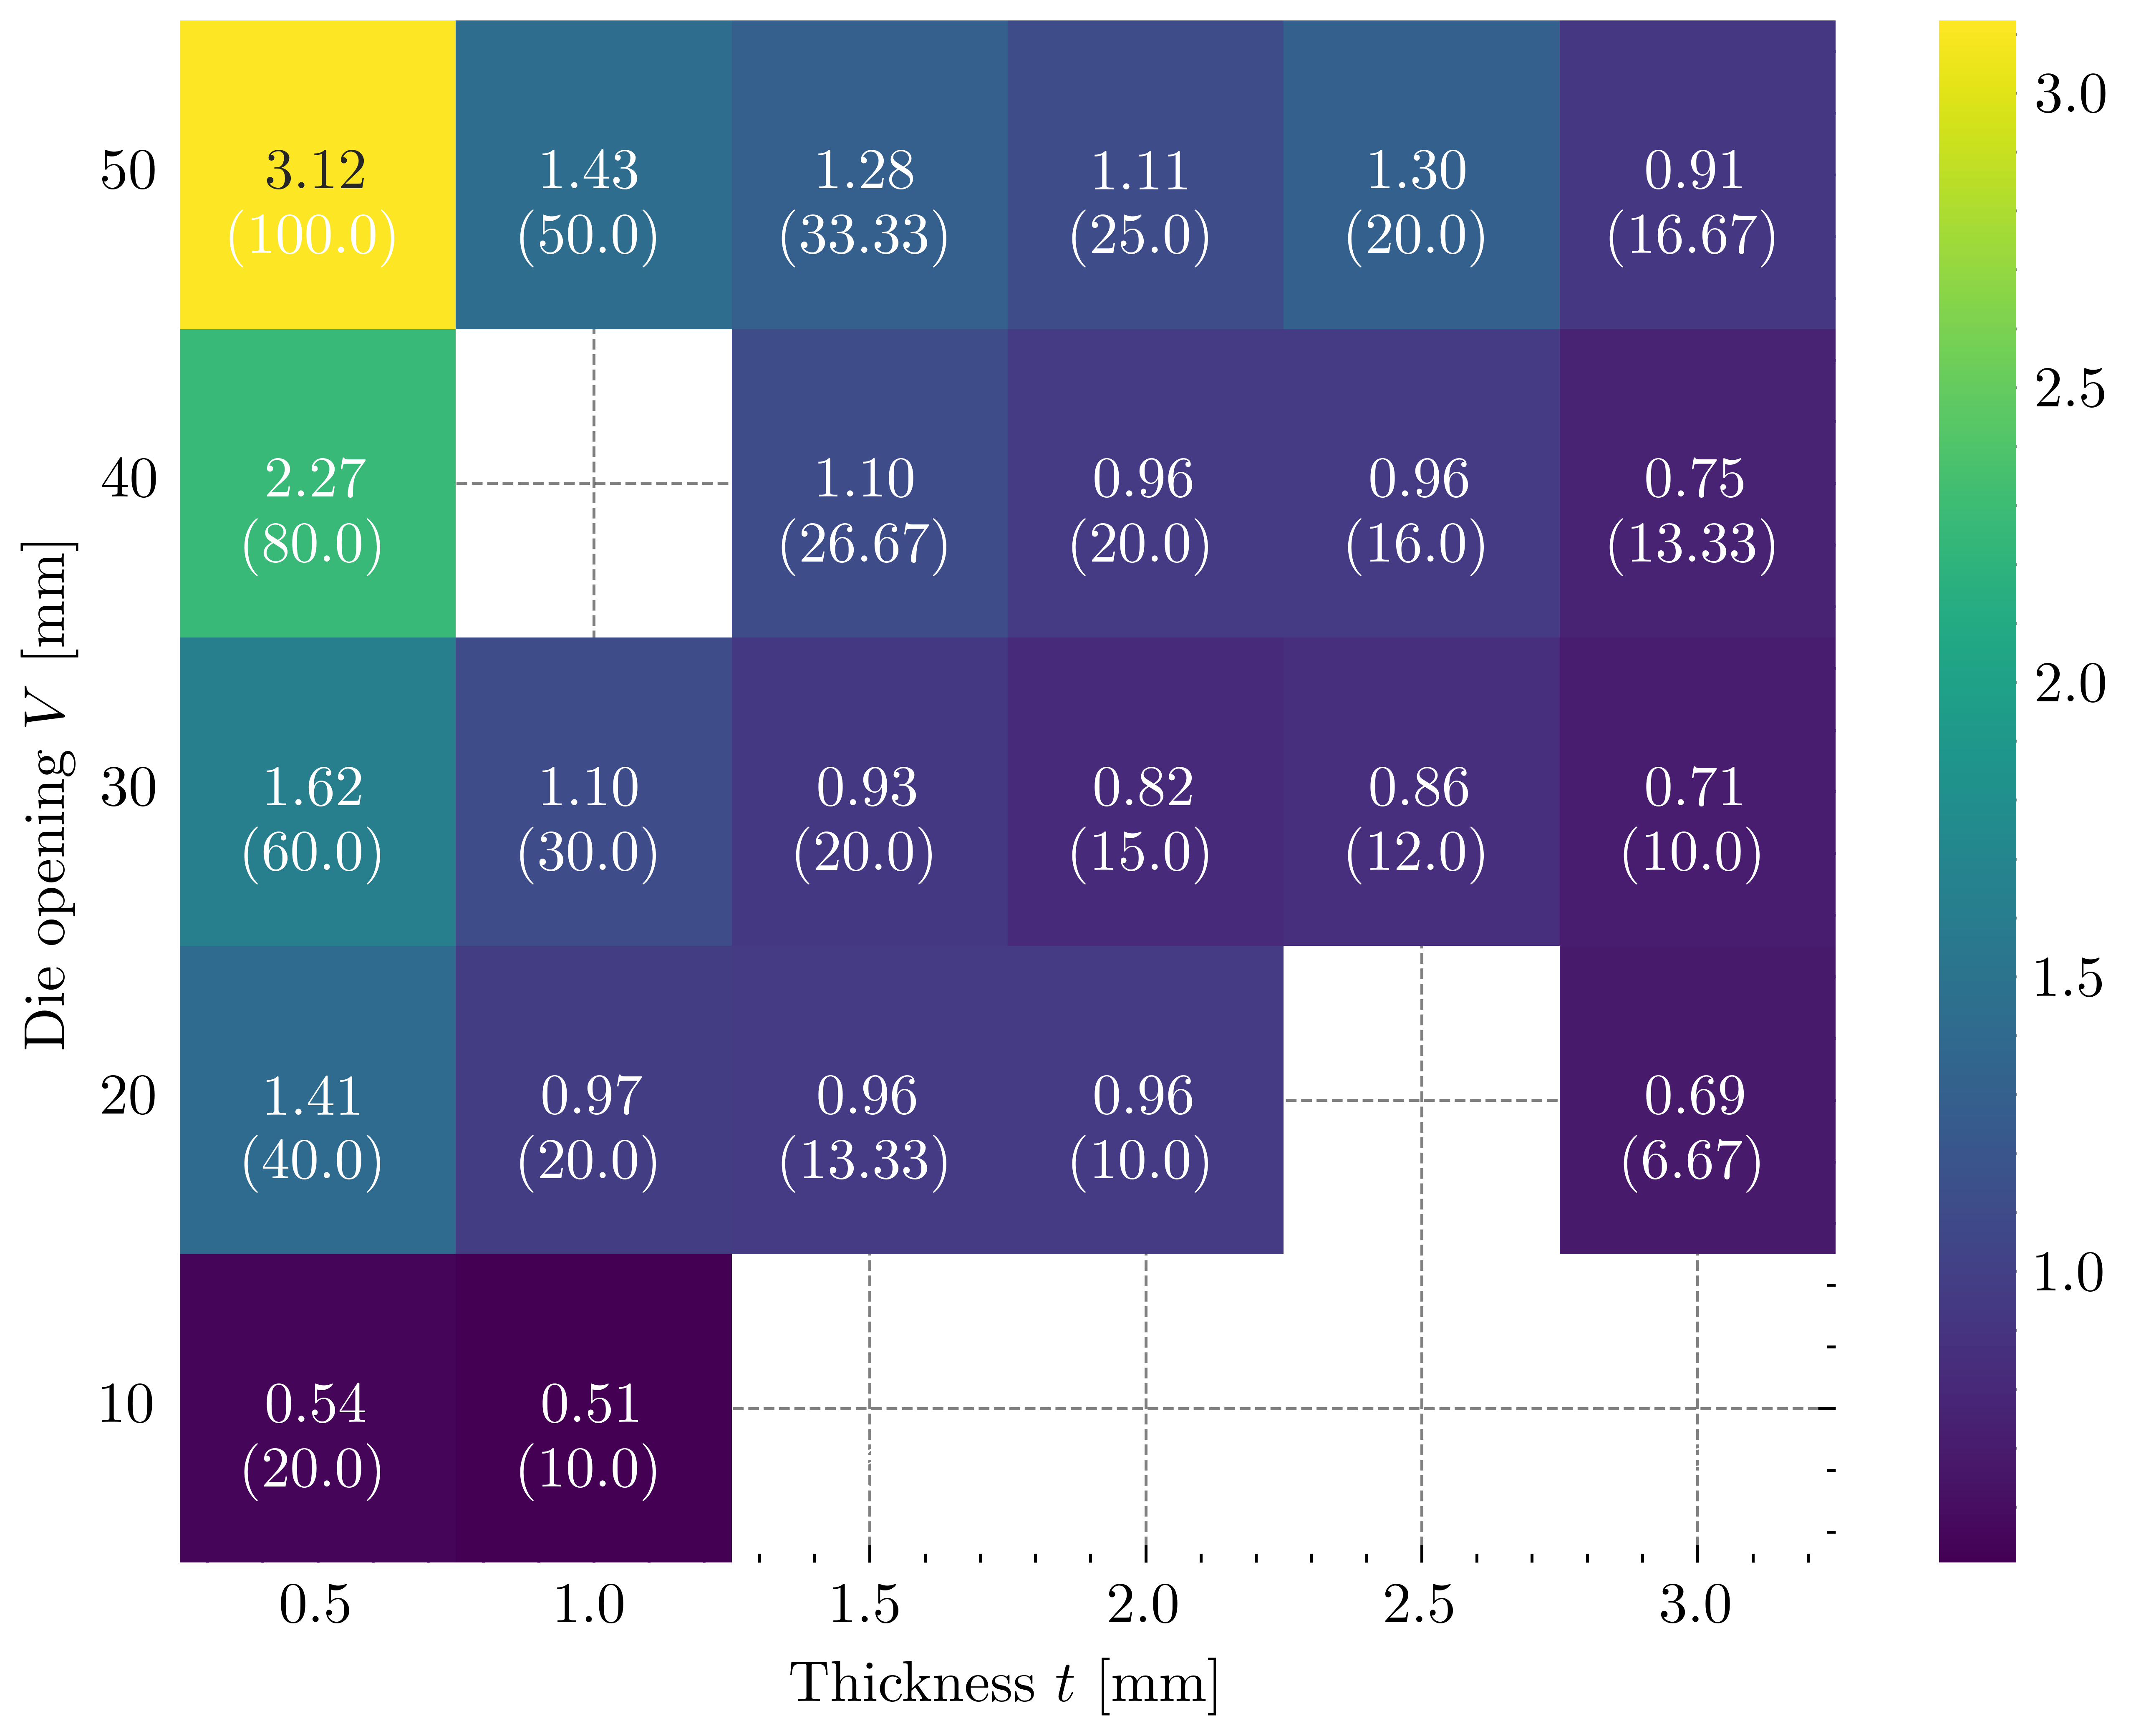
\includegraphics[width=0.6\textwidth]{chap5/images/mean_springback_heatmap}
    \end{tcolorbox}
    \caption{Mean spring back for a V/t combinations. The x-axis denoted the thickness while the y-axis denotes the
    die opening}
    \label{fig:springback-heatmap}
\end{figure}


To select specific instances for the demonstration, the V/t ratios of the instances are considered.
A V/t ratio of 20 can be considered as the the middle of the dataset. Using this as a reference, the dataset can be
divided into three cases:

\begin{itemize}
    \item Case A includes instances with low V/t ratios.
    \item Case B includes instances a V/t ratio around 20.
    \item Case C includes instances with high V/t ratios.
\end{itemize}

The chosen instances from each case are shown in \cref{tab:representative-instances}.
The two A cases represent a lower V/t ratio, the B cases represent a V/t ration between 20-30 and the C cases
represent higher V/t ratios.
More examples can be found in the accompanying CD-ROM.

\begin{table}[h]
    \begin{tcolorbox}[arc=0pt,boxrule=0.5pt]
        \centering
        \begin{tabular}{lllll}
            \toprule
            \textbf{Case} & \textbf{\(V\) } & \textbf{\(t\)} & \textbf{V/t}   & \textbf{Ratio} \\
            \toprule
            A             & 20              & 1.5            & \textbf{13.33} & low            \\
            A             & 20              & 2.0            & \textbf{10}    & low            \\
            \hdashline
            B             & 30              & 1.5            & \textbf{20}    & middle         \\
            B             & 30              & 1              & \textbf{30}    & middle         \\
            \hdashline
            C             & 40              & 0.5            & \textbf{80}    & high           \\
            C             & 50              & 0.5            & \textbf{100}   & high           \\
            \bottomrule
        \end{tabular}
    \end{tcolorbox}
    \caption{Selected representative instances A, B and C.}
    \label{tab:representative-instances}
\end{table}


\subsection{Comparison of the Models}\label{subsec:overall-comparison-model-performance}
In this section, the outcomes generated by the trained models on the selected cases A, B, and C are presented.
To ensure unbiased results, all samples that were part of the test cases were removed from the training data set.
For instance, for case A [b], all samples with a die opening of 20 and a thickness of 2 were removed from the
dataset.
This was done to prevent the models from being biased to the test cases.
It is expected that the models' overall performance will decline a since they are now trained on less data.

It is vital to remember that the target values represent the mean of all values.
While the dataset's quality is good, there may still some outliers present.
The \cref{fig:performance-case-a} depicts two chosen test cases for case A with a low V/t-ratio.
It can be seen that the models perform quite well in the prediction of the spring back.
It can be seen that all models generally follow the target values with some exceptions.
Compared with the other two cases (B and C), the models perform perform the best in case A.

\begin{figure}[hb]
    \begin{tcolorbox}[arc=0pt,boxrule=0.5pt]
        \centering
        \subfigure[a]{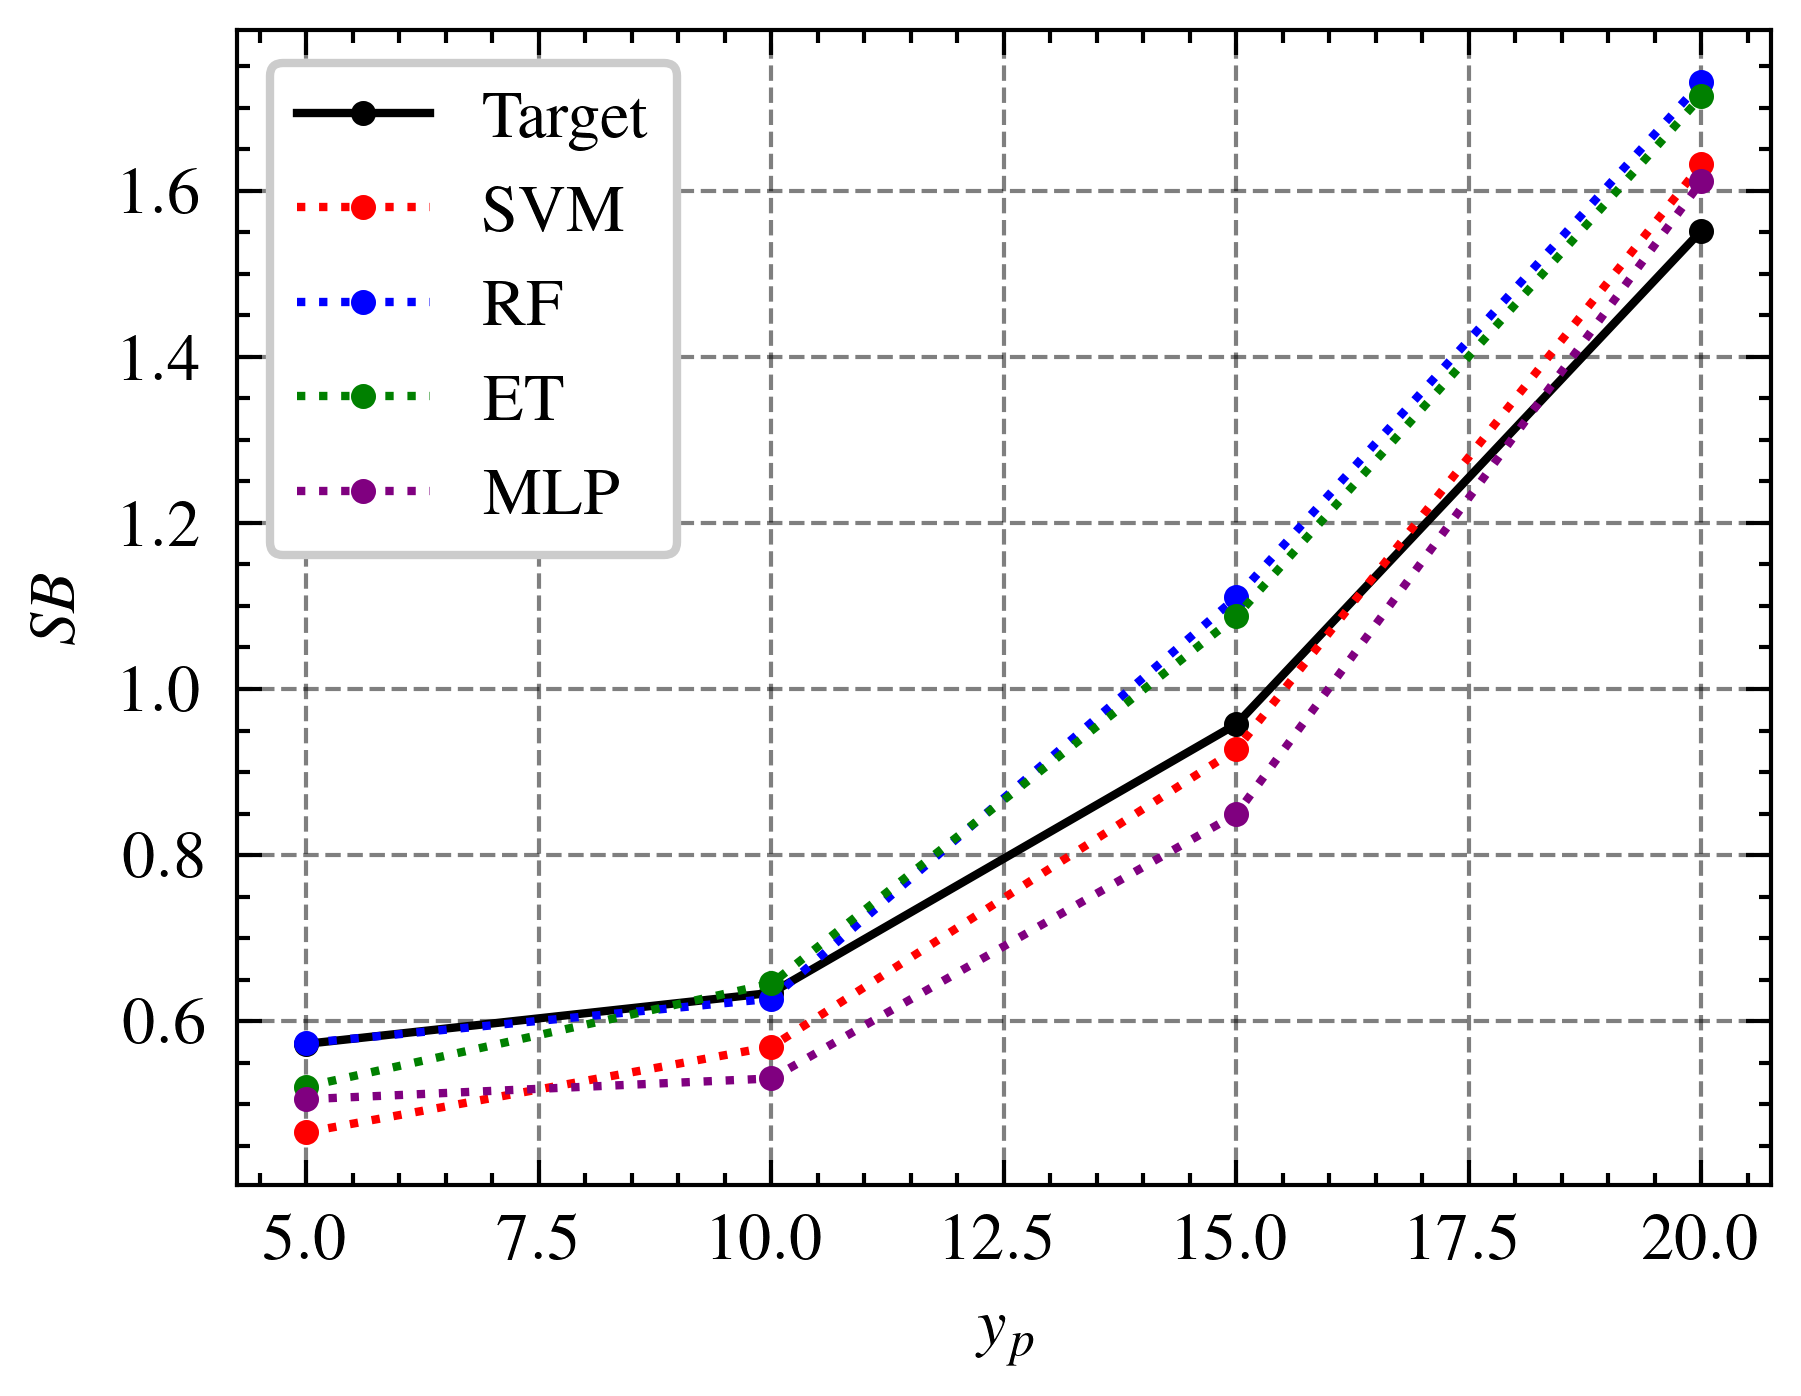
\includegraphics[width=0.4\textwidth]{chap5/images/performance_20_1.5}}
        \subfigure[b]{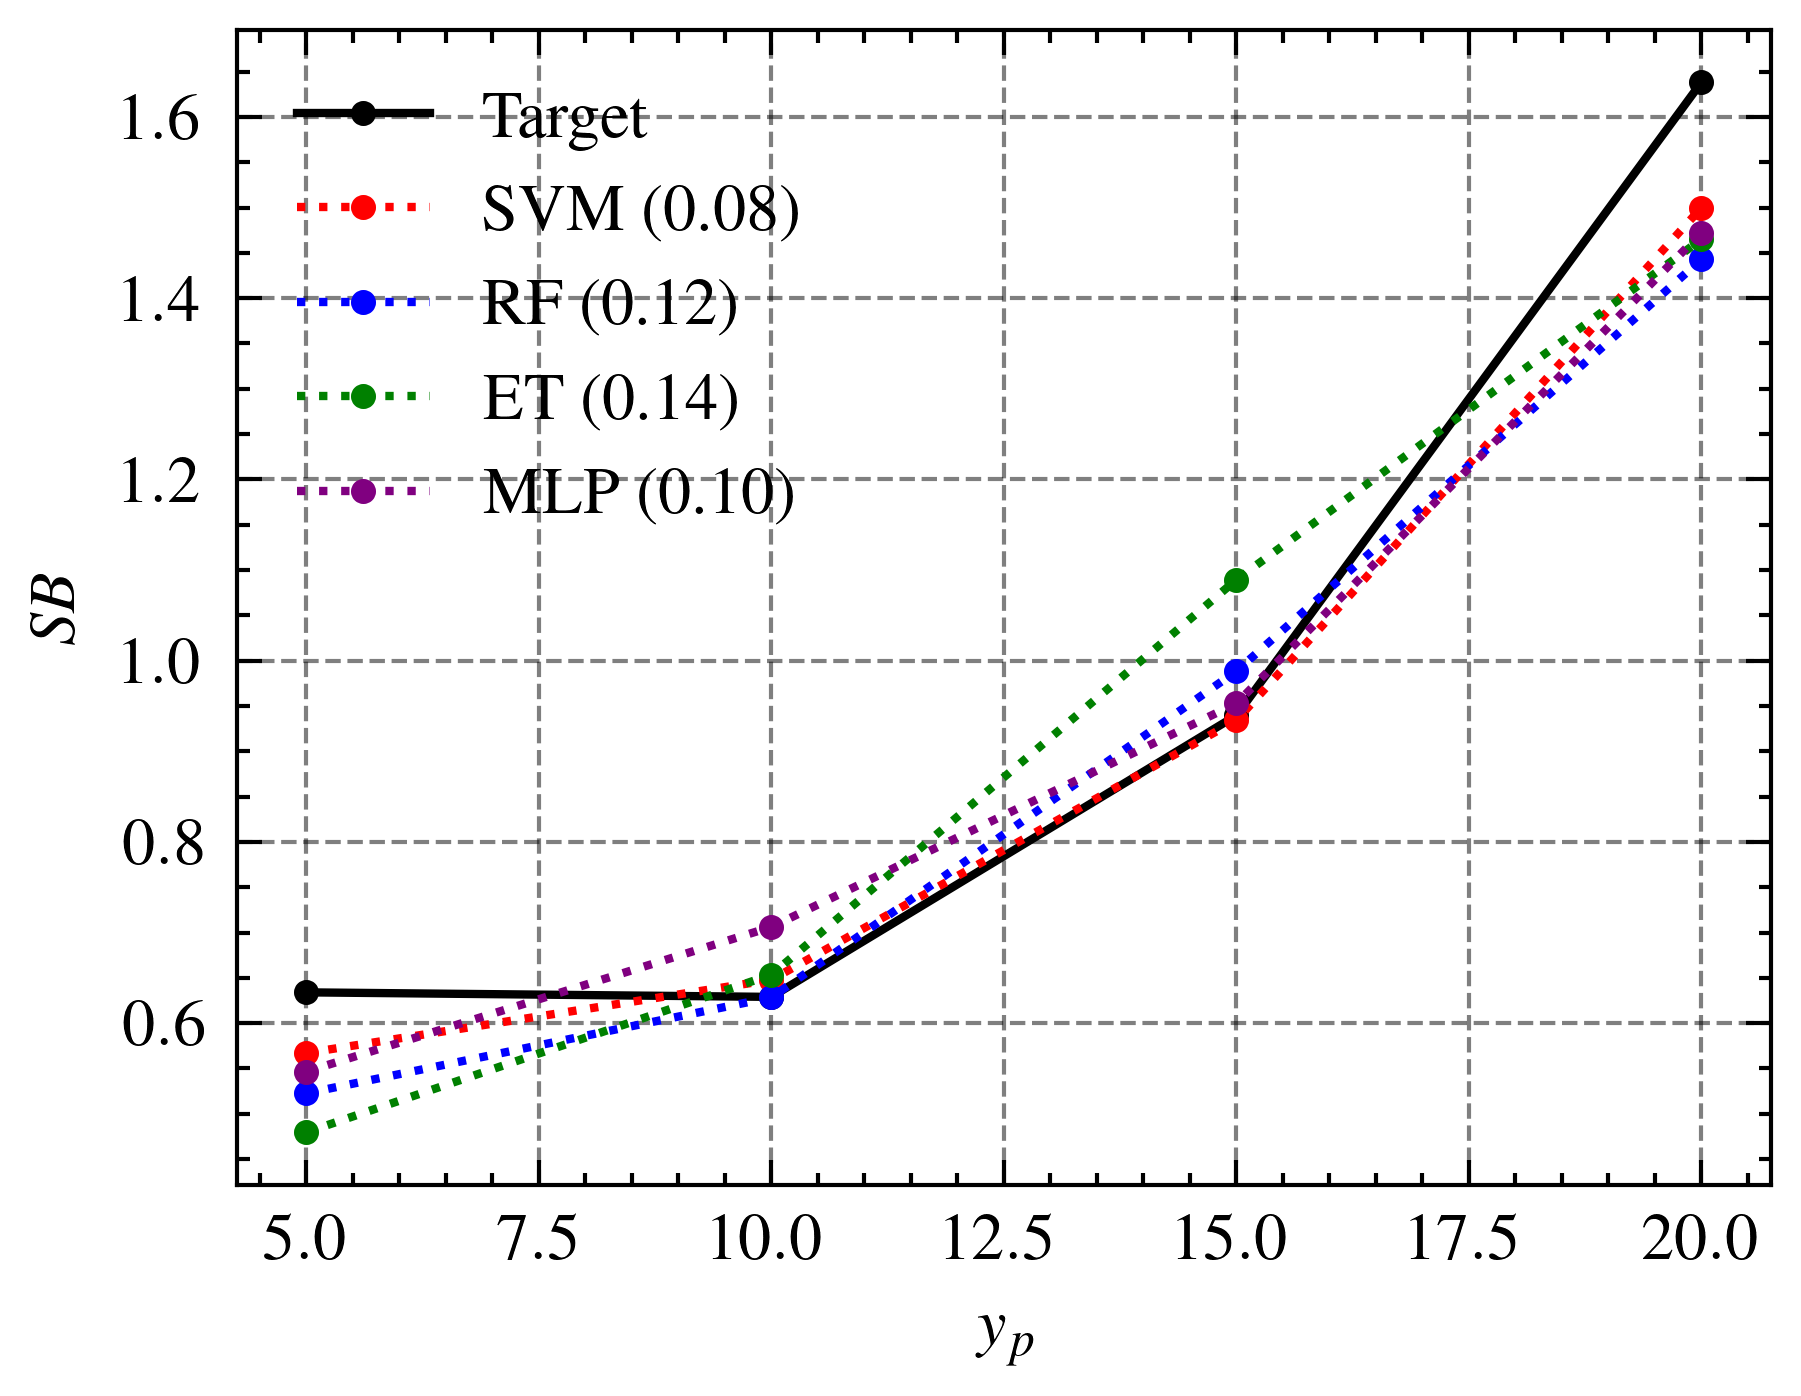
\includegraphics[width=0.4\textwidth]{chap5/images/performance_20_2.0}}
        \caption{Performance plots for case A. [a] V/t: 13, [b] V/t: 10}
        \label{fig:performance-case-a}
    \end{tcolorbox}
\end{figure}

The \cref{fig:performance-case-b} illustrates two selected instances for case B, where the V/t ratios fall within
the V/t range of 20-30.
The results give a mixed picture.
Case [a] does perform well with all models generally following the target values, with exceptions for very
low
and
very high $y_p$ values.
Case [b] on the other hand does not perform as well. It can be seen that for most $y_p$ values, the models do not
follow the target values.


\begin{figure}[h]
    \begin{tcolorbox}[arc=0pt,boxrule=0.5pt]
        \centering
        \subfigure[a]{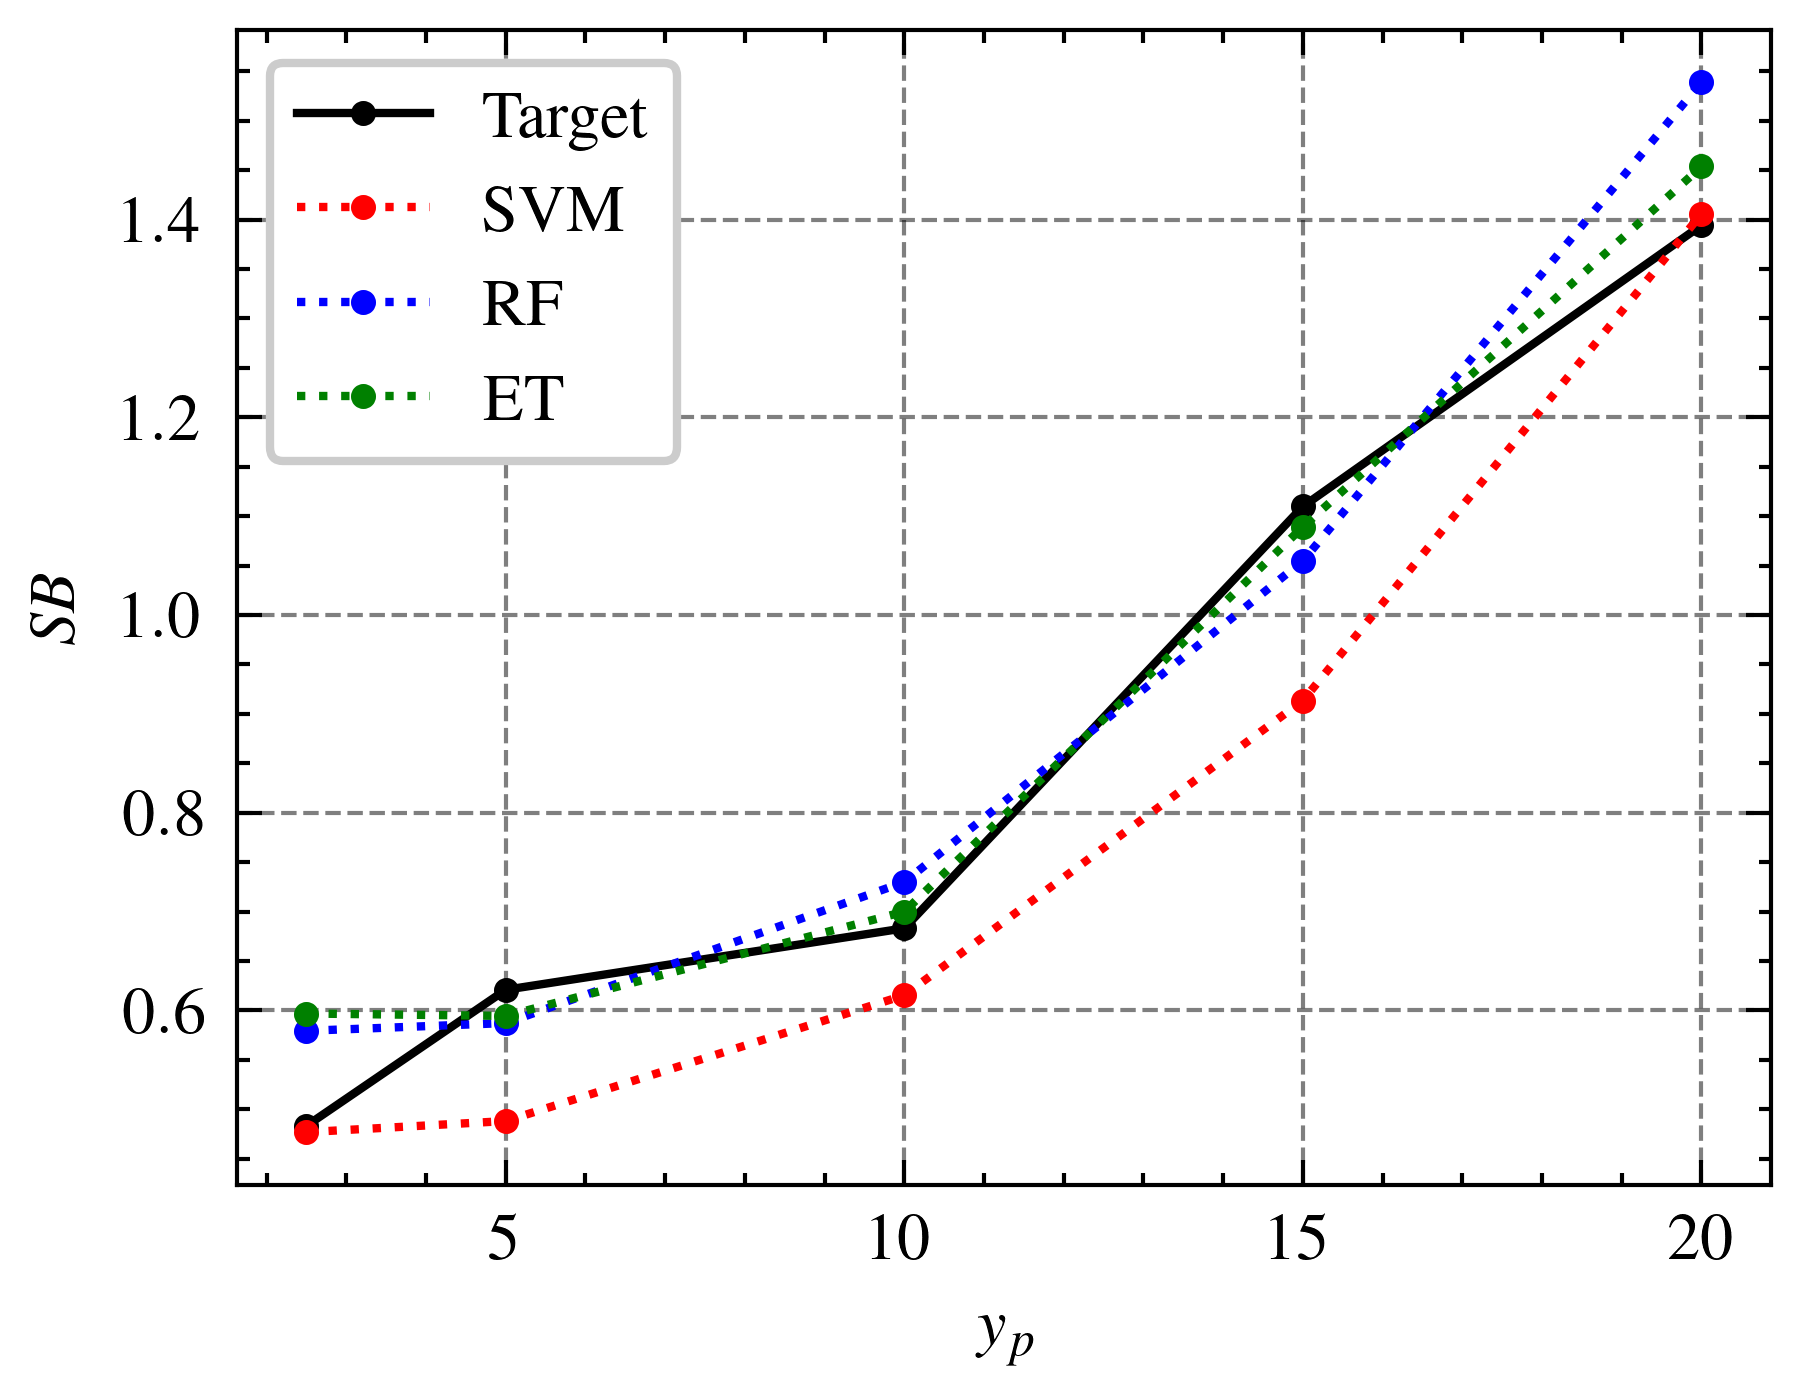
\includegraphics[width=0.45\textwidth]{chap5/images/performance_30_1.5}}
        \subfigure[b]{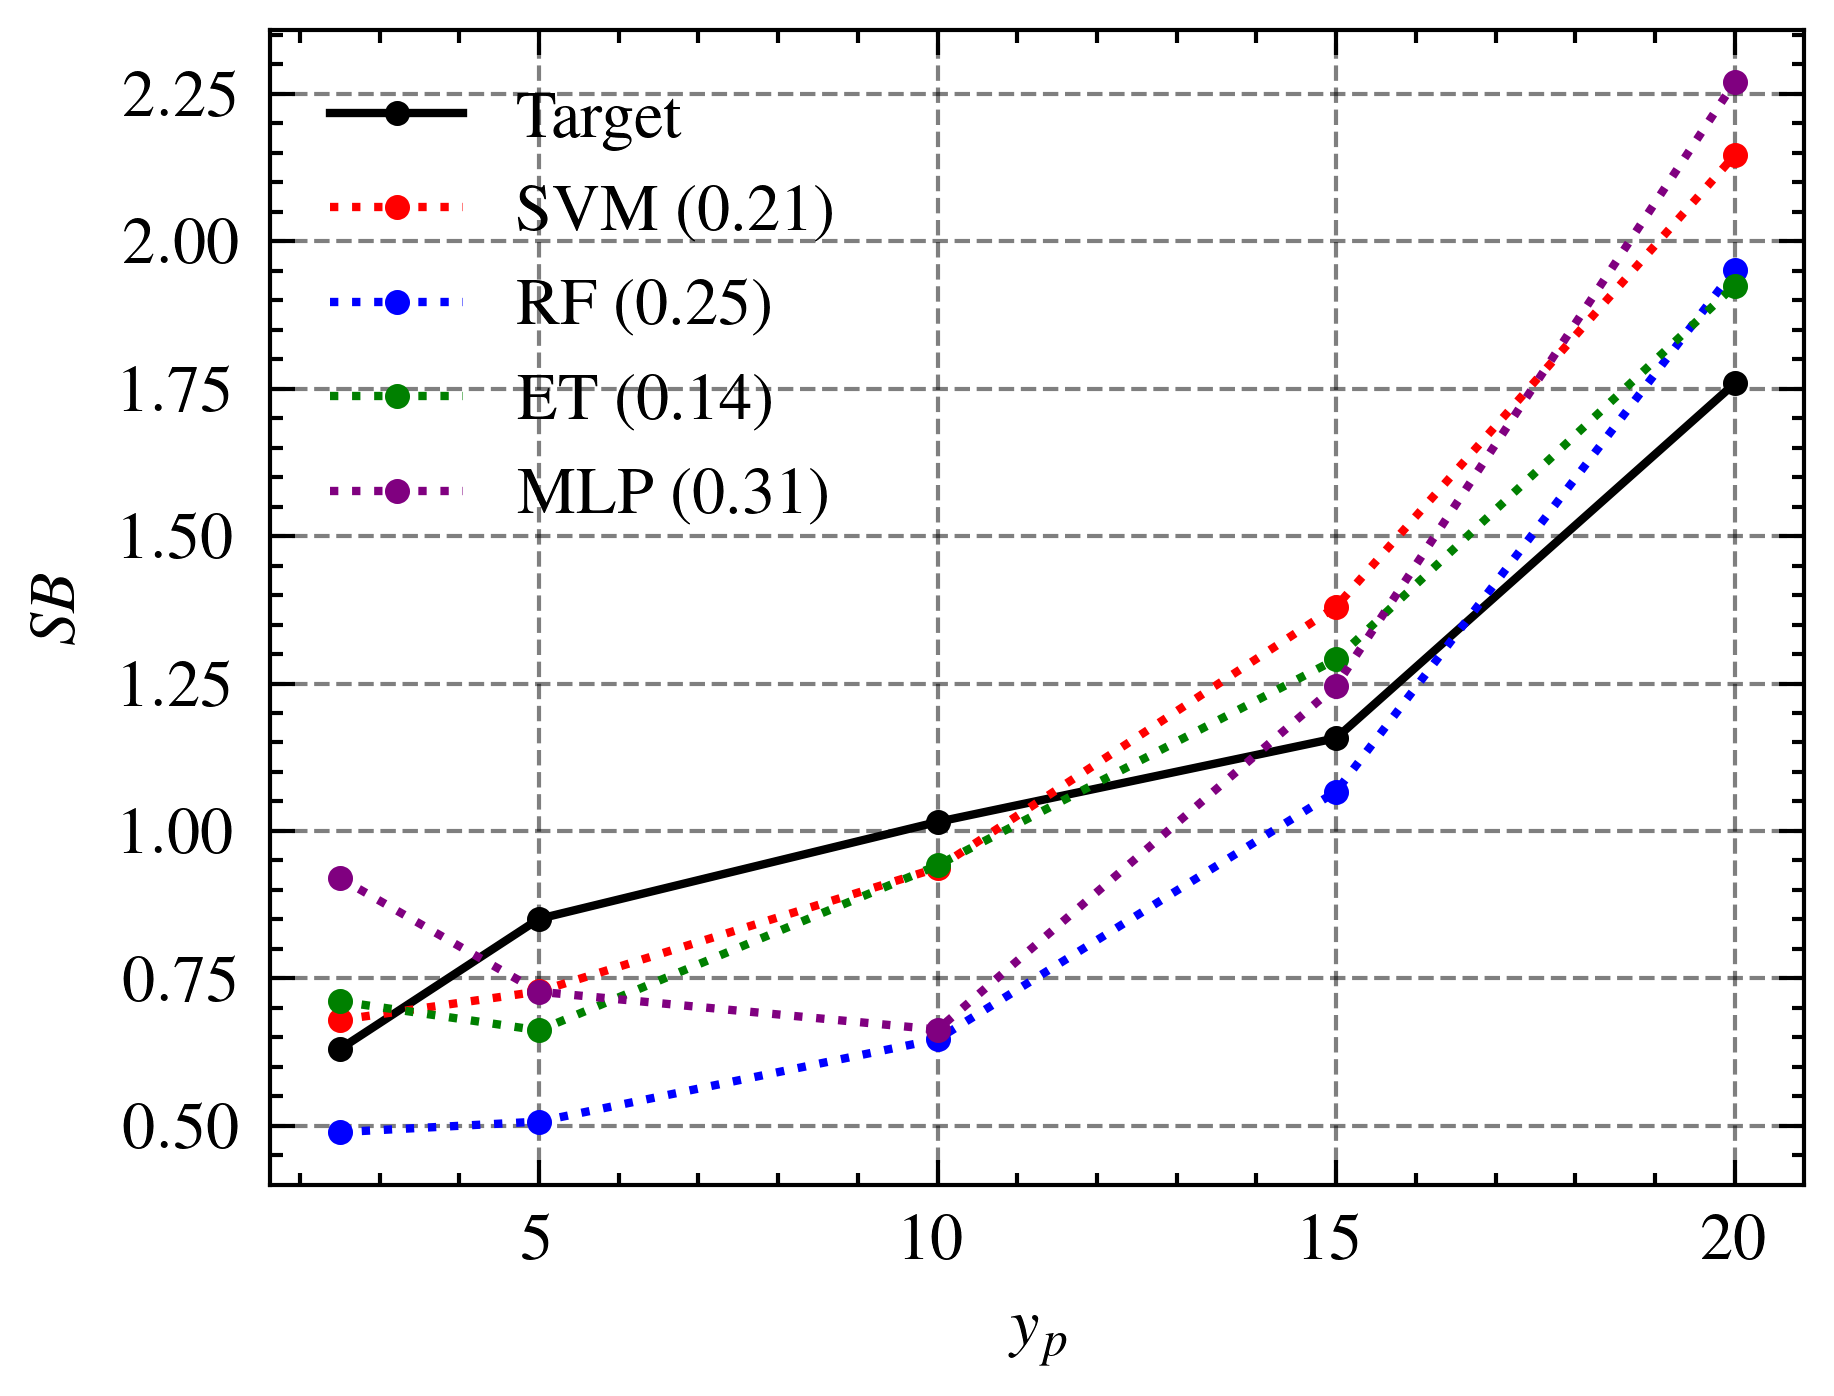
\includegraphics[width=0.45\textwidth]{chap5/images/performance_30_1}}
        \caption{Performance plots for case B. [a] V/t: 20 and [b] V/t: 30 }
        \label{fig:performance-case-b}
    \end{tcolorbox}
\end{figure}


Case C which can be seen in \cref{fig:performance-case-c} is the most challenging case, as all models exhibit visibly
poor performance.
The reason for that might be that high V/t ratios are underrepresented in the dataset and experience generally higher
spring back values.
In [a] the SVM and MLP model perform considerable better than the other models, while in [b] no good model can be
identified.
Even though the predicted spring back is bader than in the other cases, the models still are able to predict the
spring back with ~1 mm deviation in the worst case.

\begin{figure}[h]
    \begin{tcolorbox}[arc=0pt,boxrule=0.5pt]
        \centering
        \subfigure[a]{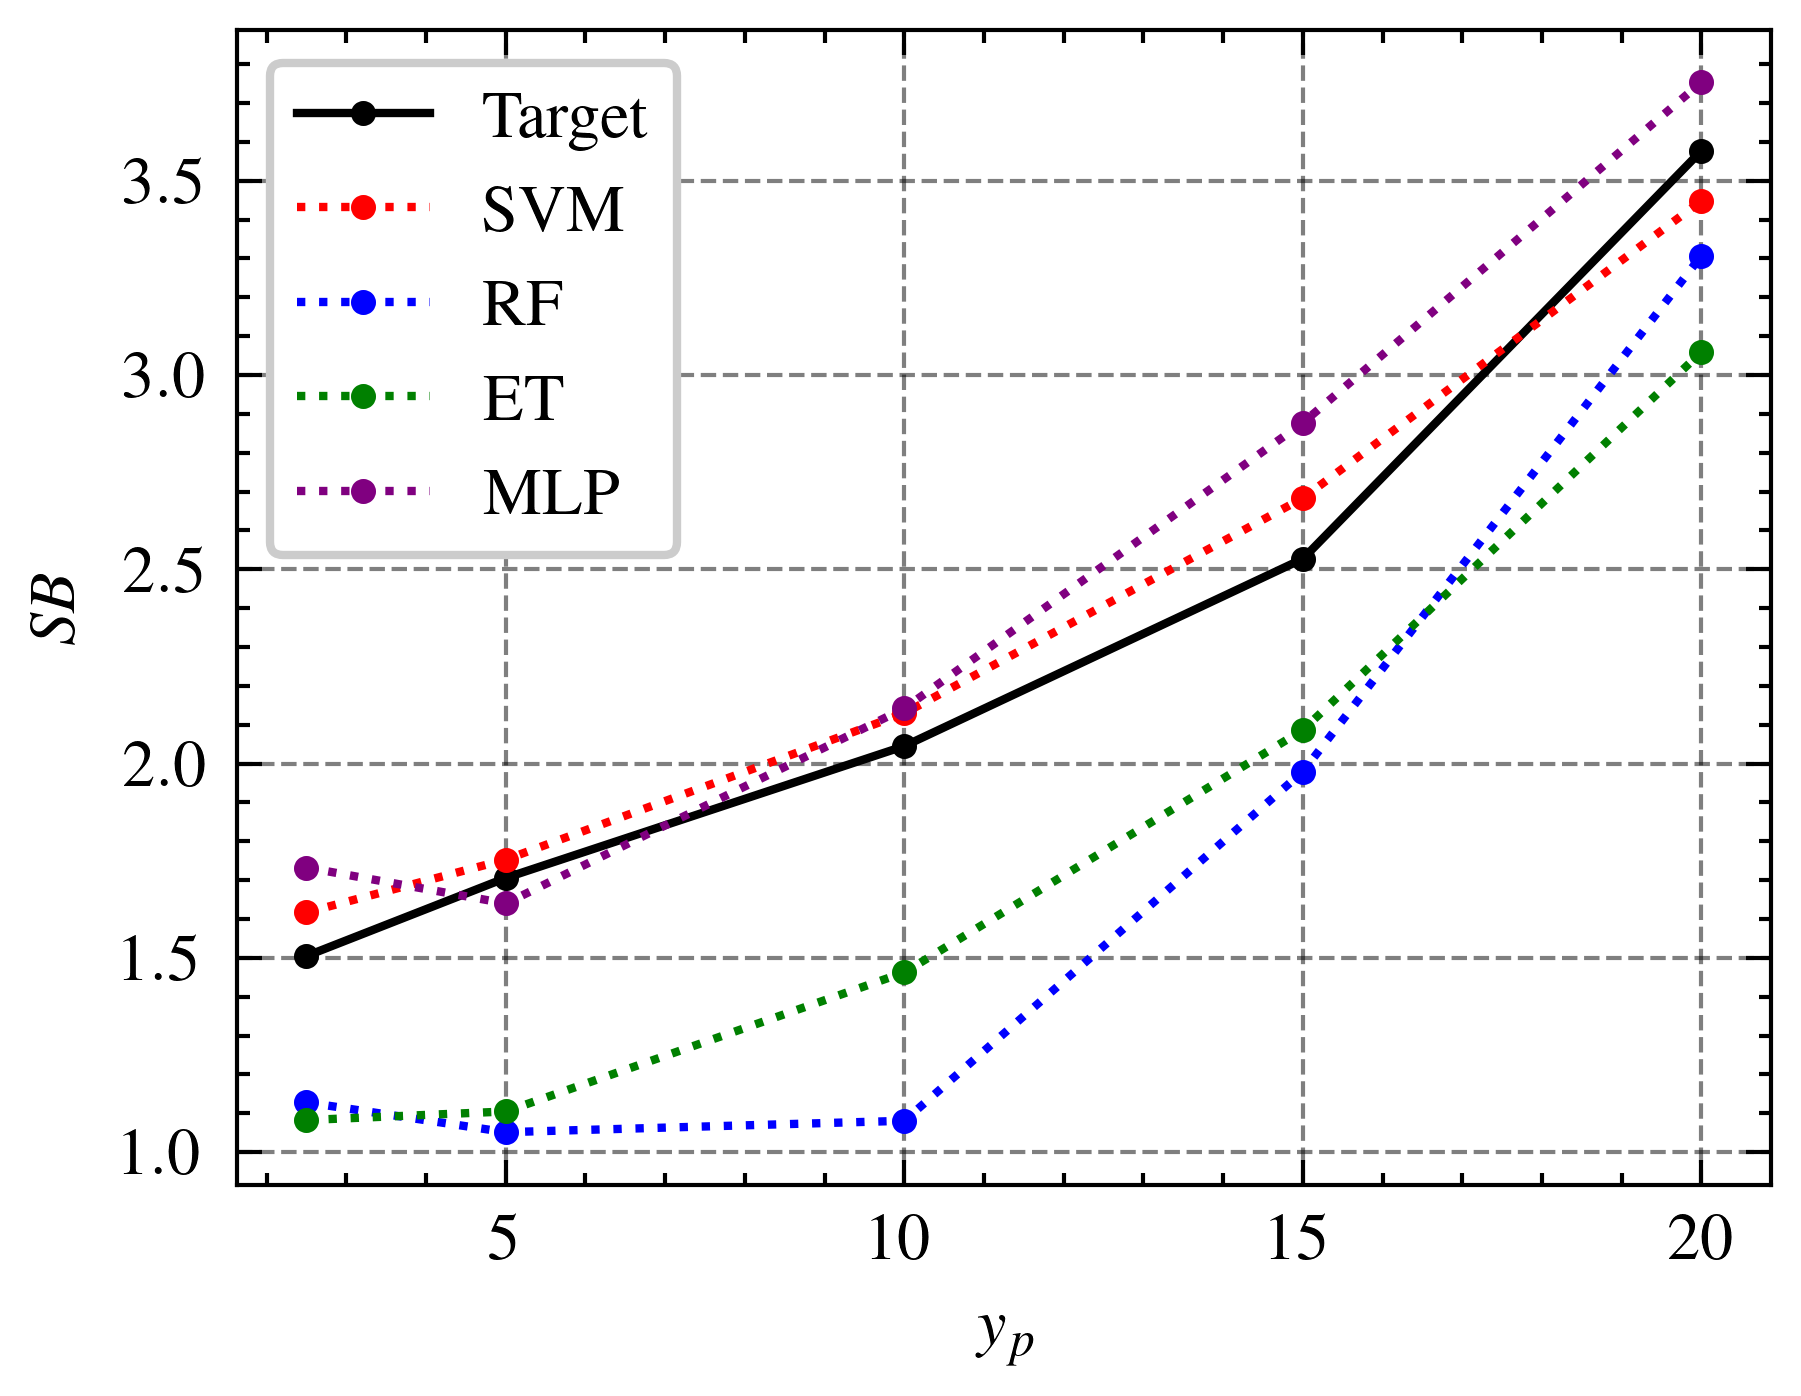
\includegraphics[width=0.45\textwidth]{chap5/images/performance_40_0.5}}
        \subfigure[b]{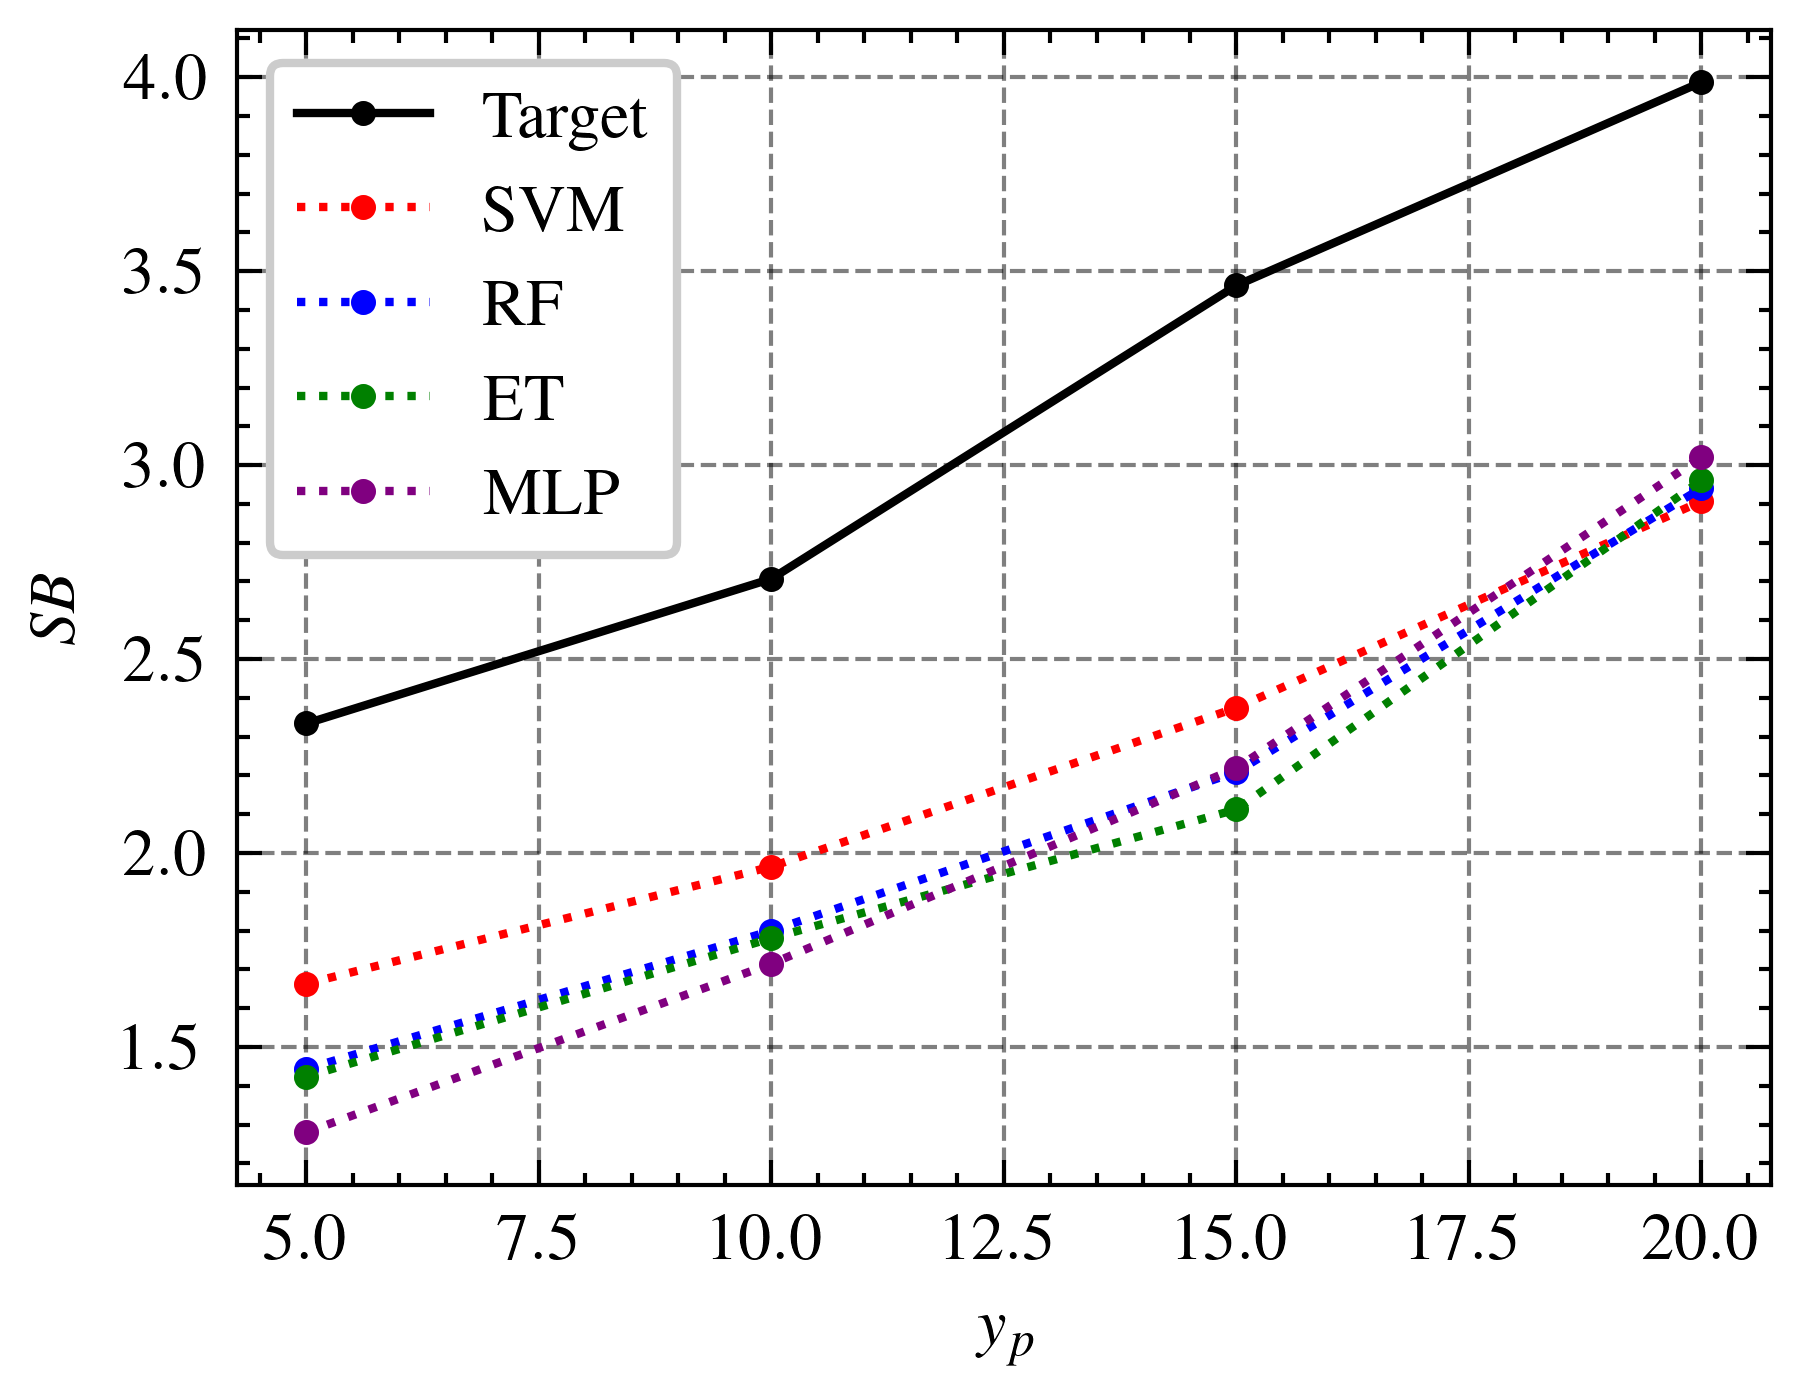
\includegraphics[width=0.45\textwidth]{chap5/images/performance_50_0.5}}
        \caption{Performance plots for case B: [a] V/t: 80 and [b] V/t: 100}
        \label{fig:performance-case-c}
    \end{tcolorbox}
\end{figure}


The best overall performing models are the \ac{MLP} and the \ac{SVM} model.
The results show that the trained models in this study do not perform good in all cases.
They seem to understimate the spring back in cases with high V/t ratios.

All models are now evaluated and presented, following the DSR process the results are interpreted and discussed in
the next sections.


\subsection{Interpretation}\label{subsec:interpretation-of-results}

The results of the this study provide insights in the applications of machine learning on the field of metal sheet
bending and the prediction of spring back.
The interpretation of the results is as follows.

\subsubsection{Hypothesis 1}
The findings support the first hypothesis that \ac{ML} models can accurately predict the spring back of bent sheet
metal parts.
The  Multi-Layer-Perceptron and Support Vector Machine models performed best with a RMSE of 0.17 mm and 0.21 mm, while
other models
still exhibited good performance.
This means that in average the predictions of the best models deviate by 0.15 mm from the actual spring back which is
a very good result.
In \cref{subsec:how-much-error-is-acceptable} it was shown that the models trained in this study are
capable of predicting spring backs with an accuracy that satisfies the highest precision level of the ISO 2768-1
standard.

Traditional trial-and-error methods, such as technology tables (refer to
\cref{sec:problem-identification-and-motivation}), offer data for a limited number of bends, encompassing
only those bends that were previously tested.
In contrast, the resulting \ac{ML} models from this study are capable of predicting an unlimited number of new bends
with high accuracy.
Therefore, it can be conclusively stated that \ac{ML} models are capable of outperforming traditional methods.

In the presentation (\cref{sec:demonstration}) it could be seen that the models do not perfom good in all cases.
In particularly they tend to underestimate high spring back values, this could be part of an area where further
research
may be needed.
To improve the prediction accuracy more data for high spring back cases might already be enough to improve the
performance to a satisfying level.

The use of real-word data instead of simulated data for the training of the models make the results of this study
more representative for real-world applications.
A comparison with other studies is challenging since variations in the bending process such as material, machine,
bending methods and other factors might yield significantly different results.
%In comparison with similar studies like \cite{baig_machinelearningprediction_2021} it can be seen that the
%real -world data used definitely paid of comparing the results

\subsubsection{Hypothesis 2}

The results show that specific \ac{ML} perform better compared to other models based on the six Design Principles
that where used.
The Support Vector Machine model demonstrated the best balance between bias and variance, but not a robust performance
when exposed to missing data and noise.
The Gradient Boosting model displayed the highest stability, while the Extra Tree and Random Forest models exhibited
the best resource utilization.
These findings suggest that selecting the most suitable ML models for specific applications is crucial for achieving
optimal performance.

Since the correctness normally has an elevates importance it can be said that the best overall performance was achieved
by the \ac{SVM} and \ac{MLP} models.
It is crucial to highlight that only a simple neural network was utilized in this study, and while it produced good
results, more complicated neural networks could produce even better outcomes.
Further more the use of ensemble models could yield interesting results (see recommendations for further
research~\ref{subsec:recommendations-for-further-research}).


\subsubsection{Hypothesis 3}
The results show that interpretability methods can provide valuable insights into factors that contribute to spring
back,
potentially leading to a better understanding of the underlying physical processes and more effective compensation
strategies.
The thickness of the metal sheet was found to have the most significant influence on spring back, while other
features, such as punch penetration and die opening, also played important roles in the models' decision-making
processes.

With he use of model-agnostic methods, the study also revealed non-linear dependencies between the input and the
target features, as well as interactions between thickness and distance.
This information can be valuable for further refining the models, as well as for developing more effective
compensation strategies in the sheet metal forming process.
This study was not able to use models with high interpretability such as decision trees or linear models
since their correctness was not good enough.

\subsection{Limitations of Research}\label{subsec:limitations-of-research}
There are some limitations to this study that needed to be considered when interpreting the results.

The dataset used has a limited number of samples, with 400 samples the models might not have enough data to capture
the full complexity of the spring back phenomenon.
Furthermore the dataset did not contain many high spring back scenarios, which might have led to the models
underestimating high spring back values.
A larger dataset with more high spring back samples could potentially improve the results.
Additionally it has to be noted that many parameters weren't changed in the experimental setup.
For example the used press brake, punch radius and material of the metal sheets where not changed.
Experiments with different bending methods and materials will most certainly yield different results.

This study had a limited number of input features (punch penetration, die opening and
metal sheet thickness).
Other potentially relevant but missing factors such as material properties, temperatures and tension might have limited
the models ability to capture all factors affecting the spring back.

Also this study had to selected a limited number of models,
there might be other models or more advanced techniques that might yield better results, recommendations for further
research will be made in the following section.


\section{Discussion of the Results}\label{sec:results-and-discussion}
The discussion is structured as follows:
The first section, titled ``Summary of Results'' presents an review of the study's findings.
The second section, ``Interpretation of Results'' delves deeper into the findings and seeks to explain them.
Both parts are structured according to the three research questions formulated
in~\cref{sec:problem-identification-and-motivation}.

\subsection{Summary of Results}\label{subsec:summary-of-results}
%Introduction
The research objective of this study is to determine whether \ac{ML} models can accurately predict the spring
back of
bent sheet metal parts.
Furthermore, the study aims to identify which model or ensemble of models performs the best.
Lastly, it seeks to utilize interpretable models to gain insights into the bending process.

The data was collected by using the air-bending process and measuring the spring back with the output data of the
press brake.
The dataset contained 400 samples, with punch penetration, die opening, and metal sheet thickness as
input features and spring back as the target feature.
The data quality was deemed good, requiring little data preprocessing.
No data imputation was necessary to achieve good results.
The data was normalized using different scalers from the sci-kit learn library.

%Key Findings

\subsubsection{Hypothesis 1}

The first research question is whether ML models can accurately predict the spring back of bent sheet metal parts.
Design Principle 1 (correctness) was used to test this hypothesis using the regression metric RMSE as the main
evaluation criterion.
The results showed that most ML models were able to predict the spring back with a RMSE of less
than 0.2 mm, indicating good accuracy.
The Multi-Layer-Perceptron and Support Vector Machine models performed best while Random Forest, and Gradient
Boosting models
demonstrated
moderate prediction
performance.
The performance of Linear Regression and Decision Tree models showed poor performance and
therefore were not considered for further analysis.


\subsubsection{Hypothesis 2}

The second research question examines whether specific ML models or ensemble models outperform other models in certain
\ac{DP}s.
\ac{DP}s 2 to 5 were used to test this hypothesis.

\textbf{Relevance:} The relevance was evaluated by assessing the bias-variance tradeoff of all trained models, except
Linear Regression and
Decision Tree.
The results showed that \ac{SVM}, \ac{ET} and \ac{MLP} have the best balance
between bias and variance and therefore were considered the most relevant.
Most models were able to explain the variance in the data.


\textbf{Robustness:} The robustness of various ML models is evaluated by examining their performance in the presence of
missing data and noise.
The experiments with missing data indicate that all models perform well when trained with 90\% of the data.
However, when trained with 50\% or less, the MLP and SVM outperform the others.

The models are also tested with added noise to the training data.
The performance of all models deteriorates rapidly as noise increases, with the first 20\% of noisy data causing the
most significant decline.
The \ac{ET} and \ac{GBT} models exhibit the most robust performance, while the \ac{RF} also demonstrates good
resilience.
Interestingly, the high-performing SVM and MLP models underperform under these conditions, likely due to overfitting
or sensitivity to outliers.

The findings emphasize the importance of using robust models and preprocessing the data to eliminate noise and
outliers.
Additionally, it was found that already more than 10\% of noise can have a significant impact on the
performance of the models.


\textbf{Stability:} The Stability was evaluated using \ac{LOOCV}.
The primary metric of the evaluation was the standard deviation of the cross-validation scores.
Here the results showed that the \ac{GBT} model was the most stable with a standard deviation of 0.183,
followed by the Extra Trees and Random Forest models.

Interestingly, the SVM and MLP models, which showed good results in other \ac{DP}s, were less stable
compared to the other models in this case.
While stability is an important factor to consider, other aspects, particularly the correctness
should also be taken into account.

\textbf{Resource Utilization:} The resource utilization was evaluated using three metrics: Training time,
prediction time and memory usage.
This metrics where used to evaluate how much computational resources the training and using a \ac{ML} model needs.

The results indicate that the \ac{ET} and the \ac{RF} with 19.541 ms and 24.912 ms had the
shortest training time compared to the other models.
The \ac{MLP} model had by far the longest training time with over 16 seconds for the relatively small dataset of 400
samples.
Regarding the inference time the \ac{GBT} model was the fastest, while the MLP again was the slowest.

In terms of memory usage the \ac{MLP} model was the most memory intensive model with 170 KB of memory usage.
The other model's memory usage was comparably low ranging from 157 KB to 159 KB.
The dataset's small size created less complex models and that contributed to the low memory usage.


\subsubsection{Hypothesis 3:} ML models with high interpretability can provide valuable insights into the factors that
contribute to spring back, potentially leading to better understanding of the underlying physical processes and
more effective compensation strategies.

To answer the third hypothesis model-agnostic methods were used to evaluate the interoperability, as model specific
method where not suitable since the used interpretable algorithm did not perform well.
Global method-agnostic methods such as feature dependence and partial dependence plots where applied to the best
performing models.

Thickness, distance and die opening where all identified as important features for the prediction spring back
with the
thickness of the metal sheet having the biggest influence on the outcome.
Partial dependence plots revealed non-linear dependencies between the features and the target variable, that was not
captured in previous research.

Additionally permutation feature importance was used to further investigate the feature importance.
The results indicate that thickness and punch penetration were crucial for the models decision-making while
the die opening did not have an impact.
This was surprising since the die opening was identified as an important feature in previous research.
To explain this finding two-way partial dependence plots where used and showed an interaction between thickness and
distance, confirming the importance of the die opening for the predictions.

Also the model-agnostic method LIME was applied to different machine learning models but did not yield any new
insights.


\subsubsection*{Further Results}
Additionally to the results found for the three hypotheses more insights where gained during the research process.
This study used the \ac{DSR} methodology to guide the research process as well as \ac{DP}s as guidelines
for
this process.
It is common for other research to use only regression metrics like MAE and RMSE for to evaluate the models.
This is understandable since the correctness of a models is usually the most important factor for the evaluation.
However, these metrics alone do not provide a complete picture of the models performance, since they do not consider
other important factors like the  \ac{ML} models this study provides a good starting point for future
research interpretability of the model or the computational resources needed to train and
predict with the model.

this study created a more comprehensive framework for the evaluation of the models by using \ac{DP}s
based on the IEEE ISO/IEC 9126 guidelines.
until a similar standard is developed for
in this field.
This framework could be used in further research to evaluate the performance of \ac{ML} models not only in the
field of
spring back prediction but also in other fields.

\subsection{How to apply the results in practise}\label{subsec:how-to-apply-the-results-in-practise}
The results show which models are best suited for a particular \ac{DP} but do not provide a clear answer to the
question of which model should be used in practice.
A general recommendation of a model is not possible since different models excelled in different \ac{DP}s, also the
prioritization of the \ac{DP}s is depending on the use case.
This study evaluates five different use cases of metal forming processes, each with different requirements and
priorities.
The following five use cases also name a concrete example industry (such as aerospace or automotive) that
could
benefit from the use of \ac{ML} models for spring back prediction.


\textbf{1. High Precision Metal Components in Aerospace Industry:}
In the aerospace industry, the importance of high precision metal components cannot be overstated.
Any inaccuracies in metal production could lead to critical failures that might endanger lives and financial
losses .
In this context, ML models that prioritize correctness, such as \ac{SVM} and the \ac{MLP}, are recommended.
These models have demonstrated their effectiveness in predicting spring back,which is essential for maintaining the
high precision required in aerospace applications.


\textbf{2. Adaptable Models for diverse Metal Components:}
When working with a wide variety of diverse metal components that differ in thicknesses, bending angles, or types of
metal, ML models need to be adaptable to these different conditions.
A relevant and stable model is essential to ensure consistent performance across different projects and should
accurately
predict the spring back for various parameters.
Among the best models in terms of relevance where the SVM, ET and MLP models.
However, the SVM and MLP models did not prove to be stable and were among the low-performing models in that regard.
Therefore, the recommended model for this use case is the ET model.


\textbf{3. Robust Models for Varying Data Quality in Automotive Industry:}
In some industries, such as the automotive industry, manufacturing with varying data quality may occur due to
factors
such as wear and tear on machinery or differences in material batches.
Therefore, a robust ML model would be essential in these scenarios, as it could handle variations in the data more
effectively.
However, the results of this study make model selection quite challenging as two tests were conducted on all models
and the top-performing models were different in each test.
In the missing values test, the MLP, followed by the SVM, where the best performing models.
However, when noise was added to the training data, a different picture emerged, with both models
performing the worst compared to the other tree-based models.
As the variance in the missing values test was not very
high,  it is advisable to prioritize the noise test.
Therefore, recommend models are the ET and GBT.


\textbf{4. Resource-efficient Models for Small-scale Manufacturing:}
There are many companies, such as small workshops, that do only small-scale metal sheet bending.
Such businesses with limited resources might want to optimize the bending process without consuming
excessive time or computational resources.
These companies want an accurate ML model that provides precise predictions while minimizing resource usage.
The results showed that the MLP consumed the most resources, while the other models had comparable performance with
lower resource consumption.
Therefore all ML models used in the study except the MLP can be recommended.


\textbf{5. Interpretability for Collaborative Projects with Non-experts:}
In many collaborative projects with non-experts, some stakeholders or users do not have a deep understanding of ML,
so it is essential that an ML model can explain its predictions.
An interpretable model can help build trust in the
model and its predictions and help identify errors in the data or the model.
In this study only model-agnostic methods where used which can be applies to any model, therefore all models can be
recommended for this use-case.


\begin{table}[h]
    \begin{tcolorbox}[arc=0pt,boxrule=0.5pt, hbox]
        \centering
        \begin{tabular}{lll}
            \toprule
            \textbf{Use case}        & \textbf{Description}            & \thead{\textbf{Recommend. models}} \\
            \midrule
            High precision           & High precision metal components & SVM, MLP                           \\
            \hdashline
            Relevant and stable      & Diverse metal components        & ET                                 \\
            \hdashline
            Robust                   & Varying data quality            & ET, GBT                            \\
            \hdashline
            Low resource consumption & Small-scale manufacturing       & All except MLP                     \\
            \hdashline
            Interpretable            & Collaborative projects          & All                                \\
            \bottomrule
        \end{tabular}
    \end{tcolorbox}
    \caption{Recommendations for \ac{ML} models based on use case.}
    \label{tab:results-in-practise}
\end{table}


\subsection{Recommendations for Further Research}\label{subsec:recommendations-for-further-research}
The limitations identified in \cref{subsec:limitations-of-research} provide direction for future research.

This study selected a limited number of \ac{ML} methods, but there are other models that could be used to
predict spring back.
Based on the results, the \ac{MLP} demonstrated superior performance in multiple \ac{DP}, indicating that
deep learning models may be promising candidates for future research.
Furthermore using ensemble models that combine the strengths for multiple other models using bagging or stacking
could
lead to interesting new results.
This would involve training multiple other models on the same dataset and combine their predictions to improve the
prediction performance and the robustness of the models.
Additionally the dataset could be expanded by adding more samples with high spring back values.
A larger dataset could potentially improve the model performance.

One of the most interesting directions for future research is the use of \ac{ML} models to predict bend deduction.
Bend deduction is the phenomenon where the metal sheet shrinks during the bending process, resulting in a smaller
piece than the one specified in the design.
Similar to the spring back this can lead to fitting issues and is therefore an important topic for further research.
As noted by~\cite{strano2017fusion}, while some prediction methods are available for spring back, bend deduction is
frequently overlooked and could be a fruitful topic for future investigation.

Moreover there are likely other factors that influence the spring back beyond those included as features in this
study.
To account for these additional patterns, future research could consider including features such as rolling
direction, temperature, and tension.